\section{Front-End Workflows}
\label{sec:FrontWorkflows}

In this section we will summarize several ``front-end'' workflows involving
the main NU-WRF model and different pre-processors. (Post-processing is
discussed in Section~\ref{sec:PostProc}). The intent is to 
illustrate the roles of the pre-processors within the NU-WRF system, and to 
show several different configurations possible with NU-WRF (e.g., advanced
land surface initialization, aerosol coupling, and CO$_2$ tracer simulation).

\subsection{Basic Workflow}
\label{subsec:BasicWorkflow}

This is the simplest approach to running simulations with NU-WRF. 
\textit{Neither chemistry nor advanced land surface initialization are 
used}, so the user should compile NU-WRF with \texttt{./build.sh wrf,wps}.

\begin{itemize}
\item \textbf{WPS}: The user must edit a \texttt{namelist.wps} file to 
customize the WRF domains, set the start and end dates, set the file formats, 
and provide information on desired terrestrial data and file prefixes.  Sample 
namelist.wps files can be found in the \texttt{WPS/}, \texttt{defaults/}, 
and \texttt{testcases/} directories. The user must then run the following 
programs [see Chapter 3 of~\cite{ref:ArwUserGuide}].

  \begin{itemize}
  \item \textbf{GEOGRID}. This program will interpolate static and 
    climatological terrestrial data (land use, albedo, vegetation greenness,
    etc) to each WRF grid. The user should use the \texttt{GEOGRID.TBL.ARW}
    located in the \texttt{WPS/geogrid/} directory to specify interpolation 
    options for each dataset selected in \texttt{namelist.wps}. (Alternative
    \texttt{GEOGRID.TBL.ARW.*} files are available for chemistry cases.)  The 
    user is also responsible for obtaining the \texttt{geog/} dataset from NCAR
    for processing by GEOGRID. Sample run scripts are available in the 
    \texttt{scripts/} directory. 
  \item \textbf{link\_grib.csh}. This script is used to create symbolic links
    to the GRIB or GRIB2 files that are to be processed. The links follow a 
    particular naming convention (\texttt{GRIBFILE.AAA}, 
    \texttt{GRIBFILE.AAB}, ..., \texttt{GRIBFILE.ZZZ}) that is required by 
    UNGRIB.
  \item \textbf{UNGRIB}. This program will read GRIB or GRIB2 files with 
    dynamic meteorological and dynamic terrestrial data (soil moisture, soil 
    temperature, sea surface temperature, sea ice, etc) and write specific 
    fields in WPS intermediate format. If necessary the user is also responsible 
    for obtaining the \texttt{GRIB/GRIB2} data and store it an appropriate file path.
    The user must select an appropriate 
    \texttt{Vtable} file in \texttt{WPS/ungrib/Variable\_Tables/} to specify 
    the fields to be extracted.
  \item \textbf{METGRID}. This program will horizontally interpolate the 
    output from UNGRIB to the WRF domains, and combine them with the output
    from GEOGRID. The user must select the \texttt{METGRID.TBL.ARW} file to
    specify the interpolation methods used by METGRID for each field. 
  \end{itemize}
\item \textbf{REAL}. This program will vertically interpolate the METGRID 
  output to the WRF grid, and create initial and lateral boundary condition
  files. REAL is described in Chapters 4 and 5 of~\cite{ref:ArwUserGuide}. 
  The user must edit a \texttt{namelist.input} file to specify the WRF domains,
  start and end times, and WRF physics configurations for REAL. 
  \emph{A standard WRF land surface model should be selected for this 
  workflow. No chemistry options can be selected.}  Sample 
  \texttt{namelist.input} files are available in the \texttt{testcases/} 
  directory.
\item \textbf{WRF}. This program will perform a numerical weather prediction
  simulation using the data from REAL. User need to change the 
  \texttt{namelist.input} file for specific run cases. A sample 
  \texttt{namelist.input} file can be found in the \texttt{WRF/run/} 
  directory and in \texttt{testcases/}. WRF is described in Chapter 5 
  of~\cite{ref:ArwUserGuide}. In addition to the normal WRF physics options, 
  the user can specify the new Goddard 3ICE or 4ICE microphysics 
  (mp\_physics=55 or 56), and the Goddard 2011, 2014 or 2017 radiation schemes 
  (ra\_lw\_physics=55, 56 or 57 for longwave, and ra\_sw\_physics=55, 56 or 57 for 
  shortwave respectively), all without aerosol coupling. Note that the 2014 radiation 
  scheme requires users to create a symbolic link to the 
  \texttt{WRF/GODDARDRAD\_SSLUT/} directory, and to put that link in the 
  directory where the model is run.  The 2017 radiation 
  scheme requires users to create a symbolic link to one file,
  \texttt{WRF/run/BROADBAND\_CLOUD\_GODDARD.bin}, and to put that link in the 
  directory where the model is run.

  A feature added to NU-WRF is the calculation of mean integrated
  vapor transport. The user may adjust the time-averaging period for this
  diagnostic by changing the IVT\_INTERVAL flag in the 
  \&time\_control block of \texttt{namelist.input}. A value of 0 indicates
  instantaneous values will be output as the ``means'', while positive
  values indicates averaging time periods in minutes.
  
\end{itemize}
\centerline{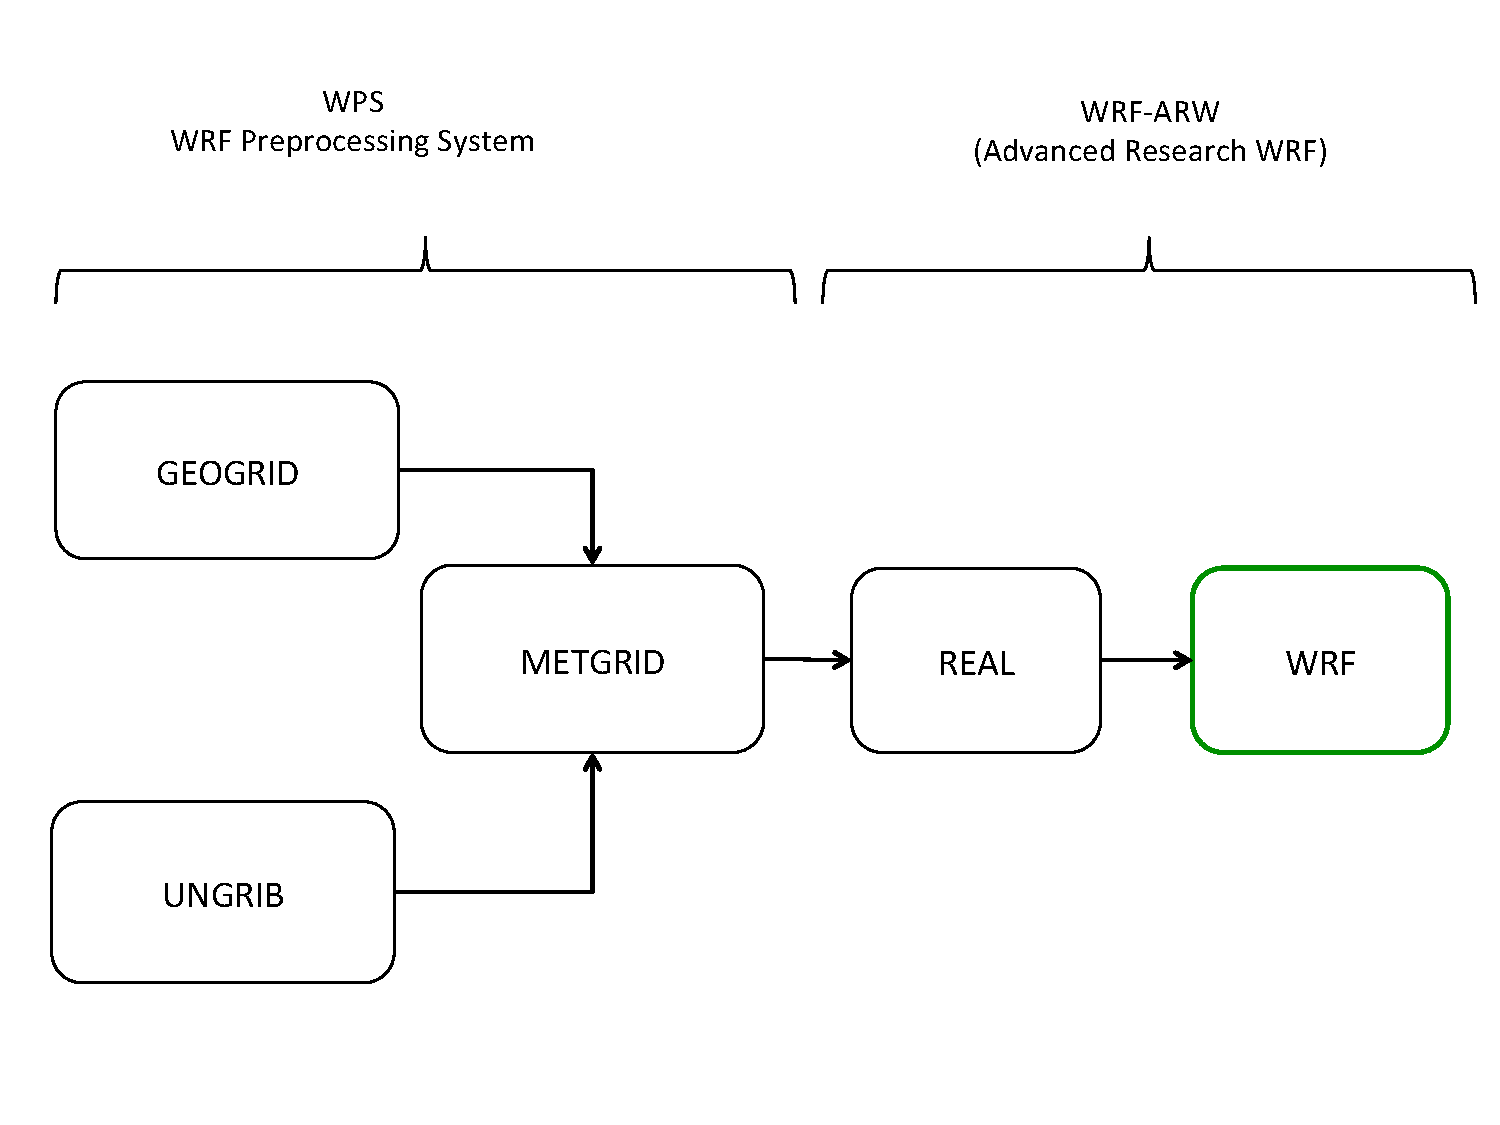
\includegraphics[width=4.5in]{basic-workflow}}

\subsection{Land Surface Initialization and LIS Coupling}
\label{subsec:LisWorkflow}

This is a more advanced approach to running simulations with NU-WRF. Instead
of using land surface fields interpolated from a coarser model or reanalysis,
a custom-made land surface state is created by LIS on the same grid and with
the same terrestrial data and land surface physics as WRF.  WRF will then
call LIS on each advective time step, providing atmospheric forcing data
and receiving land surface data (fluxes, albedo, etc) in return. 

For simplicity, this workflow uses no chemistry,  so the user should compile 
NU-WRF with \texttt{./build.sh wrf,wps,lis,ldt,lisWrfDomain}. However, an 
advanced user can combine this workflow with one of the chemistry workflows 
described further down; in that case, the user should replace the \texttt{wrf}
target with \texttt{chem} (or with \texttt{kpp} if using KPP-based chemistry).

\begin{itemize}
\item \textbf{WPS}. These steps are identical to those WPS steps in 
Section~\ref{subsec:BasicWorkflow}.
\item \textbf{LISWRFDOMAIN}. The user must provide a \texttt{ldt.config} file 
  (used by LDT) and a \texttt{lis.config} file (used by LIS).  The LISWRFDOMAIN 
  software will read the \texttt{namelist.wps} file and the netCDF4 output 
  files from GEOGRID, and copy the WRF grid information to the two 
  configuration files. LISWRFDOMAIN is divided into two executables: 
  \texttt{lisWrfDomain} (a Fortran compiled program found in 
  \texttt{utils/bin/}) and \texttt{lisWrfDomain.py} (a Python wrapper
  script found in \texttt{utils/lisWrfDomain/scripts/}).  

  The software can be run as 
  \texttt{./lisWrfDomain.py DOMAINPROG LISCONFIG LDTCONFIG WPSDIR}, 
  where \texttt{DOMAINPROG} is the path to \texttt{lisWrfDomain}, 
  \texttt{LISCONFIG} is the path to \texttt{lis.config},
  \texttt{LDTCONFIG} is the path to \texttt{ldt.config},
  and \texttt{WPSDIR} is the directory containing \texttt{namelist.wps}
  and the GEOGRID netCDF4 output files.

  Sample configuration files are provided in \texttt{defaults/} and in 
  \texttt{testcases/}.

\item \textbf{LDT}. The user must further customize the \texttt{ldt.config}
  file and a separate parameter attributes file to specify the static 
  and climatological terrestrial data to be processed in ``LSM parameter 
  processing mode'' [see~\cite{ref:LdtUserGuide}].  For NU-WRF Version 9, the 
  following settings are recommended/supported:
  \begin{itemize}
  \item Noah.3.6 is the recommended land surface model (Noah 3.3, 3.2, or 2.7.1
    can also be used);
  \item MODIS is the recommended land use dataset (UMD and USGS are also 
    supported);
  \item SRTM30 is the recommended terrain elevation dataset (GTOPO30 is also
    supported);
  \item STATSGOFAO is the recommended soil texture dataset;
  \item NCEP monthly climatological albedo and and max snow free albedo are
    recommended;
  \item NCEP monthly climatological and maximum/minimum vegetation greenness
    are recommended; 
  \item NCEP slope type is recommended;
  \item Use of the ``slope-aspect correction'' is recommended to improve
    soil moisture spin-ups; and
  \item ISLSCP1 deep soil temperature with terrain lapse-rate correction is
    recommended (not using the lapse rate correction could result in warm
    biases in high terrain).
    
  \end{itemize}

\item \textbf{LIS}. The user must further customize \texttt{lis.config} for 
  a ``retrospective'' run.  This includes specifying the start and end dates 
  of the ``spin-up'' simulation, identifying the LDT datasets, specifying the 
  land surface model, and identifying the atmospheric forcing datasets. The 
  user must also customize a forcing variables list file compatible with
  the forcing dataset, and a model output attributes file. All these files
  are described in more detail in ~\cite{ref:LisUserGuide}.  (Recall that
  only Noah 2.7.1, Noah 3.2, Noah 3.3, and Noah 3.6 can be used with NU-WRF).
  Sample forcing variable and output attribute files are provided in the
  \texttt{testcases/} directory.

\item \textbf{LDT}. After running LIS, it is necessary to rerun LDT in ``NUWRF
preprocessing for real'' mode. This requires modifications to 
\texttt{ldt.config} to specify the static output file from LDT and the dynamic
output file from LIS. Fields from both will be combined and written to a new
netCDF output file for use by REAL.  Sample files are given in 
\texttt{testcases/}.

\item \textbf{REAL}. REAL is run similarly to the configuration in Section
~\ref{subsec:BasicWorkflow}, except that it also reads the static and dynamic
land surface data collected by LDT. For this to work, the 
\texttt{namelist.input} file must include an additional namelist block:

\begin{quotation}
  \&lis

    lis\_landcover\_type = 2,

    lis\_filename = ``lis4real\_input.d01.nc''

  /
\end{quotation}

Here lis\_landcover\_type specifies the land use system used with LIS and LDT
(1 = USGS, 2 = MODIS, 3 = UMD), and lis\_filename is an array of character
strings specifying the combined LDT/LIS files for each WRF domain.

In addition, the user must specify LIS as the land surface model selection
with WRF (sf\_surface\_physics=55). 

The resulting initial and lateral boundary conditions will replace the 
land surface fields from UNGRIB with those from LDT/LIS. 

\item \textbf{WRF with LIS}. Running WRF in this case is similar to the
basic case in Section~\ref{subsec:BasicWorkflow}, except that WRF will 
also read the \texttt{lis.config} file and the LIS restart files that were
produced during the ``retrospective'' run. The user must modify 
\texttt{lis.config} to run in ``WRF coupling mode'', and specify 
\texttt{forcing\_variables\_wrfcplmode.txt} as the forcing variables list file.
The start mode must also be changed to ``restart'', and the time step for
each LIS domain must match that used with WRF (specified in 
\texttt{namelist.input}).

\end{itemize}

\centerline{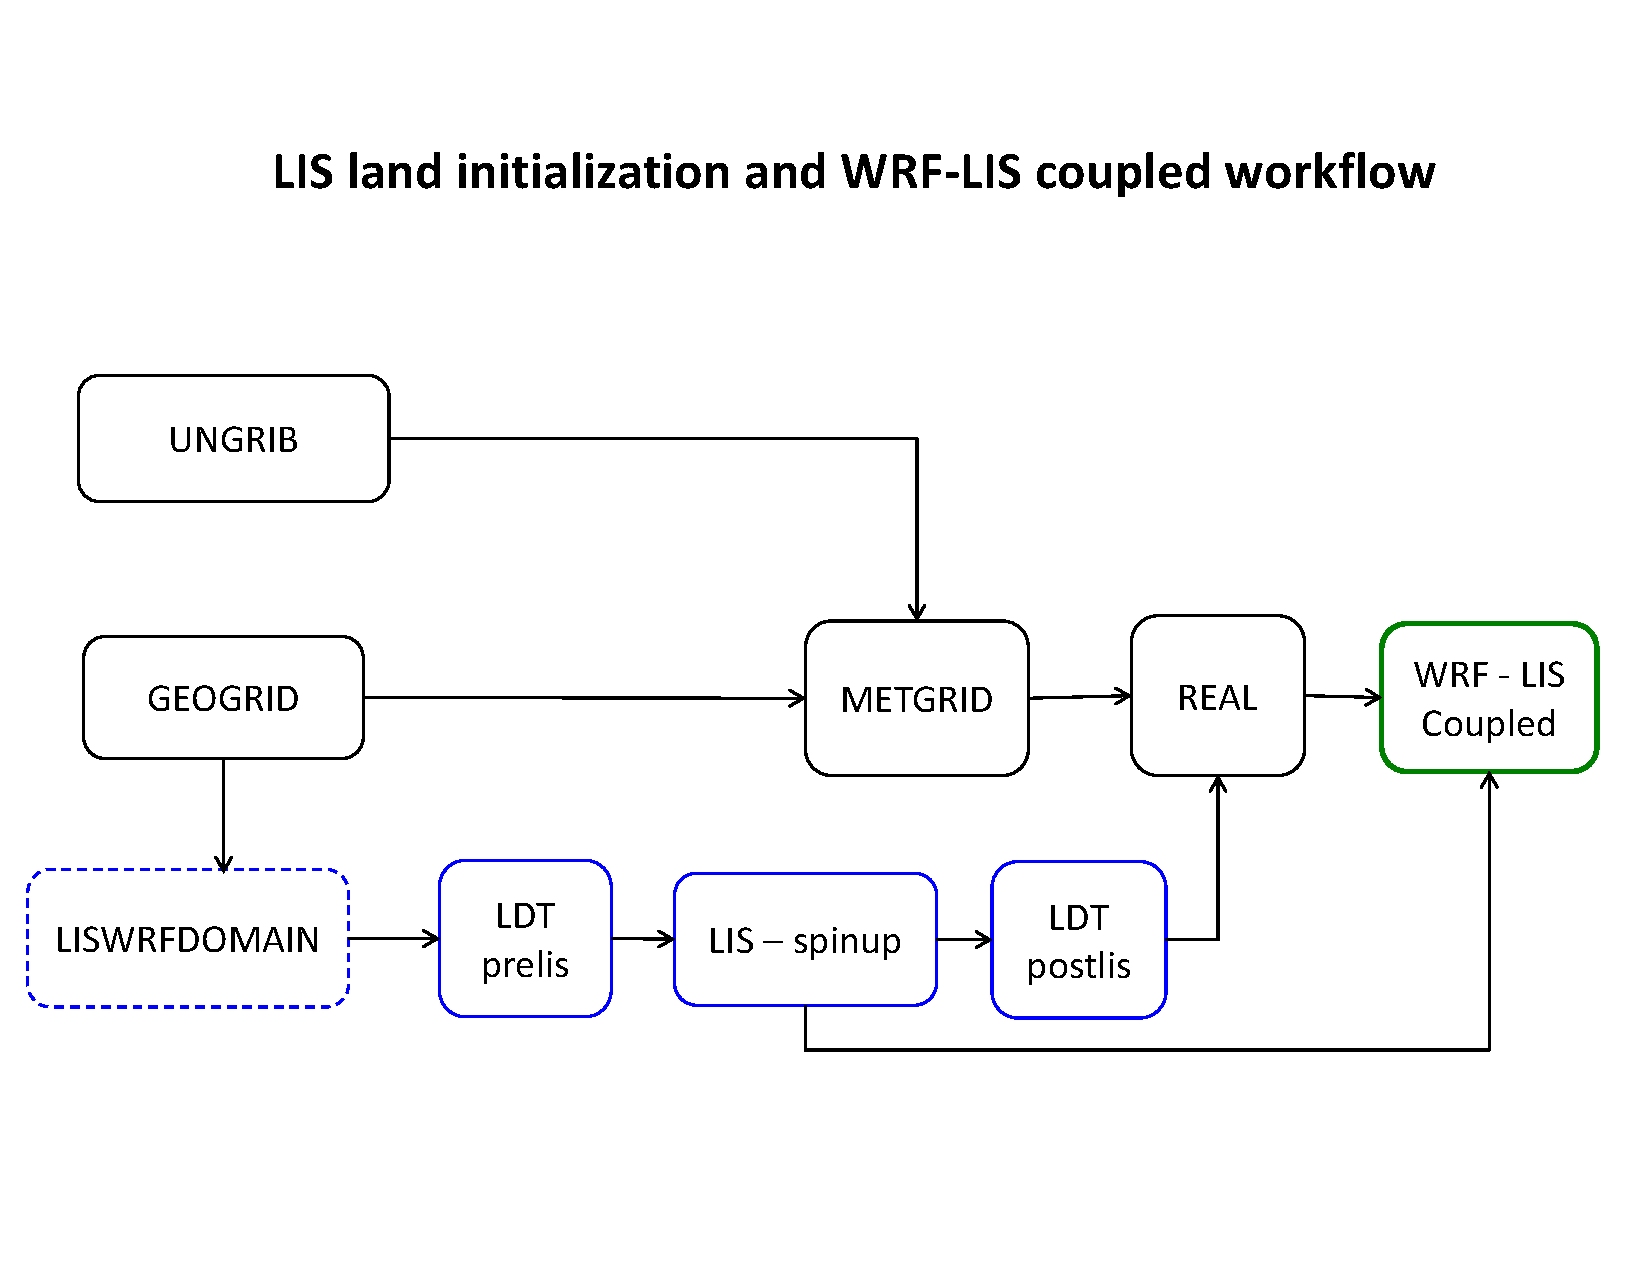
\includegraphics[width=5.0in]{LIS_workflow}}


\subsection{Single Column Model with LIS Coupling}
\label{subsec:ScmLisCoupling}

Recently, an idealized configuration for WRF with LIS coupling was added to
NU-WRF:  the \emph{WRF-LIS Single Column Model} (SCM) mode.  Based on the 
community SCM mode, the WRF-LIS SCM configuration runs with a $3 \times 3$ 
staggered horizontal grid ($2 \times 2$ for the unstaggered mass grid) and 
horizontally homogeneous initial conditions.  Boundary conditions are 
periodic.  To run the WRF-LIS SCM, the system must be compiled using
\texttt{./build.sh ideal\_scm\_lis\_xy,wps,lis,ldt,lis4scm}, followed by this
workflow:

\begin{itemize}

\item \textbf{GEOGRID}.  Run GEOGRID in a $3 \times 3$ staggered grid centered
on a point of interest.  Any normal map projection can be used (i.e., Lambert
Conformal, Mercator, or Polar Stereographic), but the spatial grid resolution
should be small ($\sim1$ km) to make the projection approximately Cartesian.

\item \textbf{UNGRIB}.  Run UNGRIB to extract initial conditions from a 
suitable external dataset.

\item \textbf{METGRID}.  Run METGRID to merge the GEOGRID and UNGRIB output 
together.

\item \textbf{BUILD\_SCM\_FORCING}.  Configure and run 
\texttt{build\_scm\_forcing.bash} in \texttt{testcases/wrflis/scm}.  This
shell script runs the \texttt{build\_scm\_forcing.ncl} script under the hood,
which extracts column initial conditions and writes them in
\texttt{profile\_init.txt} and \texttt{surface\_init.txt}.  (Advanced 
options also exist to generate forcing data and ensemble perturbations, but
these have not been tested yet.)

\item \textbf{LDT}.  Run LDT in ``LSM parameter processing mode''.  Use a
$2 \times 2$ unstaggered grid with the point of interest at the center of the 
\emph{southwest grid box}.  A latitude-longitude map projection can be used,
but the grid spatial resolution should match that of GEOGRID.

\item \textbf{LIS}.  Run LIS in ``retrospective'' mode using the same grid
configuration as LDT.

\item \textbf{LDT}.  Rerun LDT in ``NUWRF preprocessing for real'' mode.

\item \textbf{LIS4SCM}.  Edit the \texttt{namelist.lis4scm} file in 
\texttt{utils/lis4scm/input/} to enter (1) the name of a LIS restart file 
generated by the retrospective run, (2) the output file generated by LDT when 
preprocessing for real, and (3) the parameter file generated by LDT for LIS.  
Then run LIS4SCM.  This program will modify the three data files and make them
horizontally homogeneous by copying the values in the southwest corner to the 
remainder of the grid.

\item \textbf{IDEAL}.  Edit a \texttt{namelist.input} file:  
  \begin{itemize}

    \item Make sure to specify a $3 \times 3$ grid and the same spatial 
      resolution used by GEOGRID.
    \item Make sure to set \texttt{io\_form\_auxinput3} to zero in namelist 
      block \texttt{\&time\_control} (unless using idealized forcing, which 
      has not been tested).  
    \item Make sure to set the \texttt{\&lis} namelist block settings to use 
      the output file generated by LDT for real after it has been modified by
      LIS4SCM.
    \item Make sure to set the \texttt{\&scm} namelist block [see Chapter 5 of
      \cite{ref:ArwUserGuide}].  Note that the settings for land use,
      soil type, vegetation fraction, and canopy water are ignored, as these 
      are provided by LDT and LIS.
    \item Make sure to set \texttt{periodic\_x} and \texttt{periodic\_y}
      in the \texttt{\&bdy\_control} namelist block to ``.true.''.
    \item Make sure to set \texttt{pert\_coriolis} in \texttt{\&dynamics} to
      ``.true.''.
    \item Make sure to set \texttt{sf\_surface\_physics} in the 
      \texttt{\&physics} namelist block to 55 (indicating LIS on-line 
      coupling).
  \end{itemize}

  When complete, run the IDEAL program in \texttt{WRF/test/em\_scm\_lis\_xy/},
  using only a \emph{single} processor.  This will produce a wrfinput file.

  \item \textbf{WRF with LIS}.  Run WRF with the wrfinput file produced by
    IDEAL and the LIS and LDT file homogenized by LIS4SCM.  Make sure to use
    a \emph{single} processor.  Otherwise, follow the instructions in section
    \ref{subsec:LisWorkflow}

\end{itemize}

\centerline{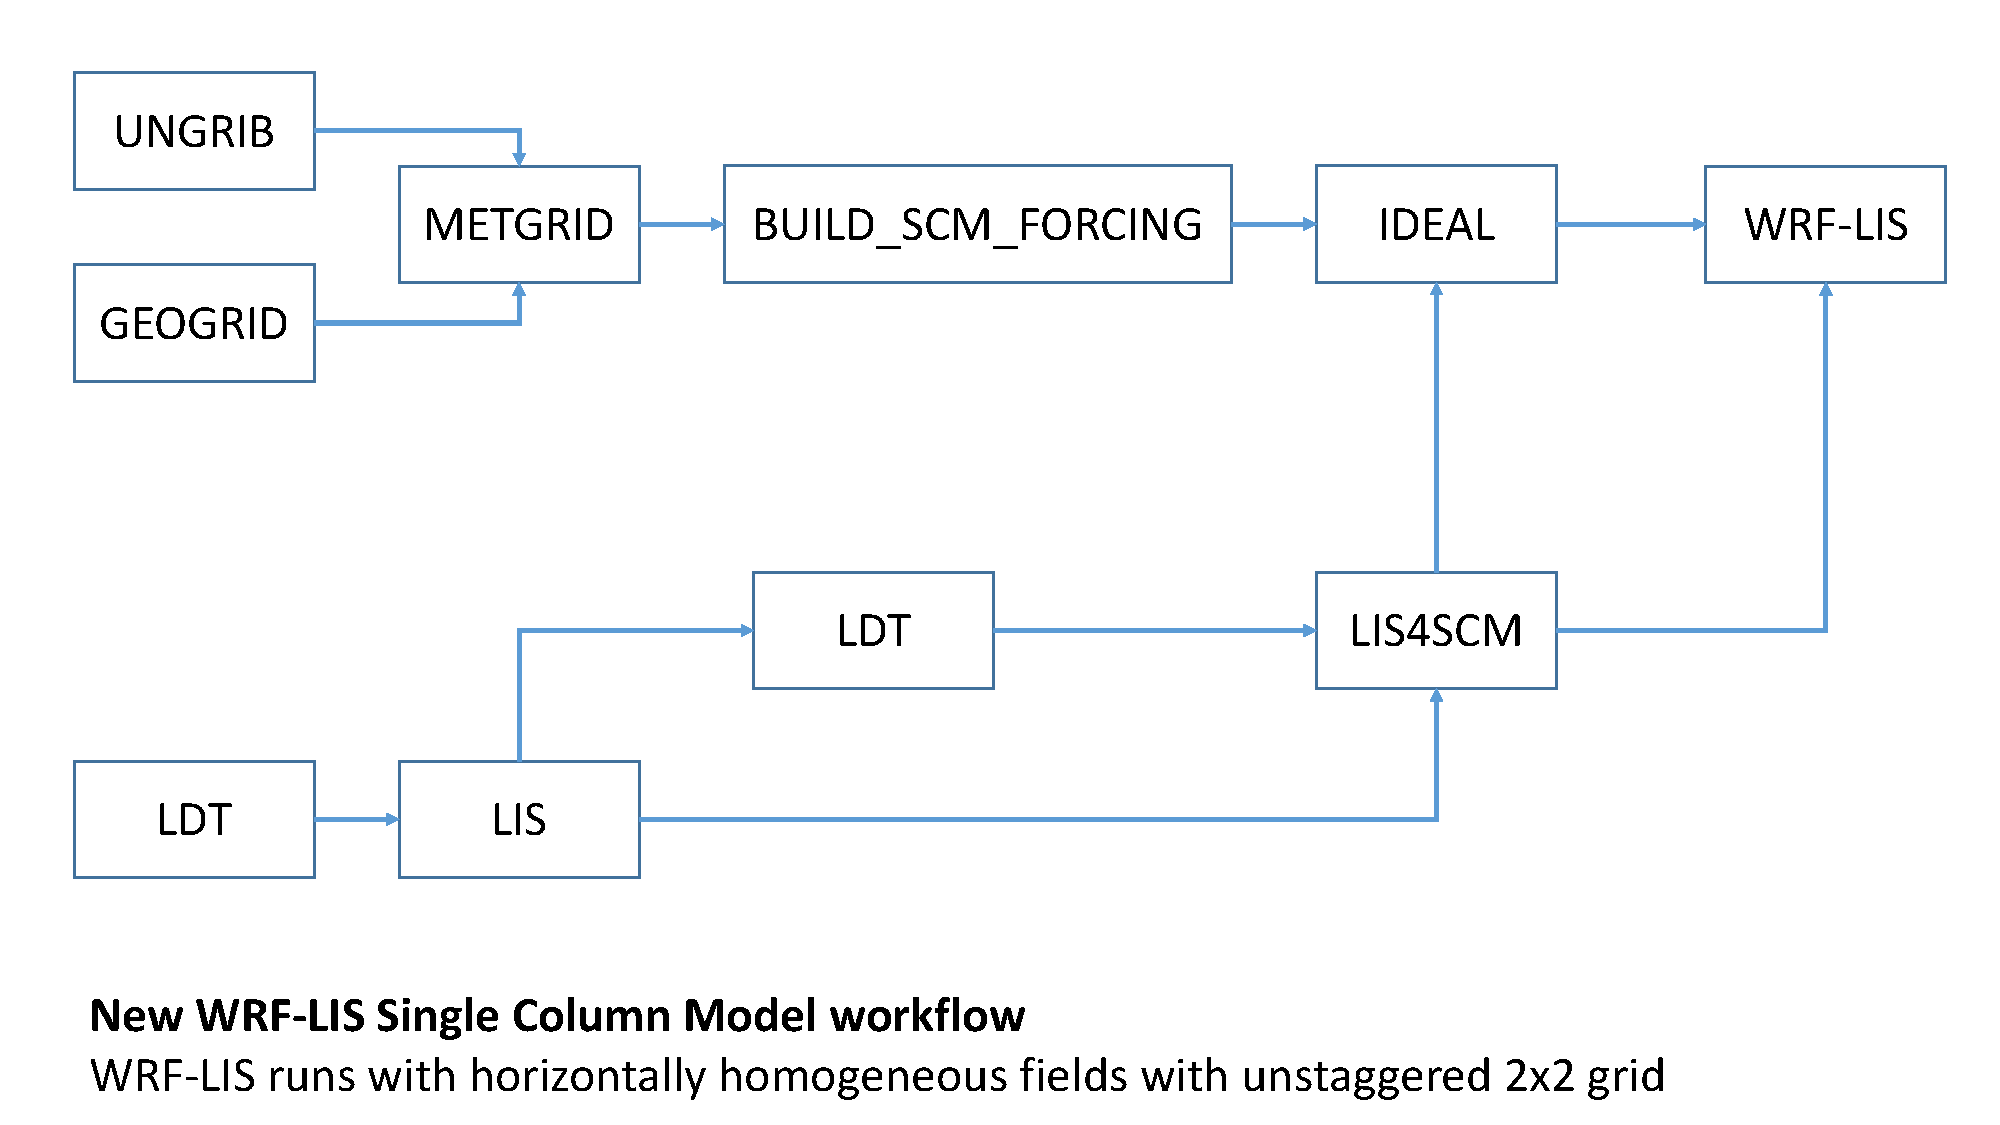
\includegraphics[width=4.5in]{wrf_scm_workflow}}

\subsection{Use of GEOS-5 Meteorological Data}
\label{subsec:Geos5}

One source of initial and lateral boundary conditions is NASA's GEOS-5 
global model~\citep{ref:RieneckerEtAl2008}. A number of dataset options
exist from GEOS-5, including daily near-real-time simulations 
(see \url{http://gmao.gsfc.nasa.gov/products}), and archived 
MERRA~\citep{ref:RieneckerEtAl2011} and
MERRA-2~\citep{ref:BosilovichEtAl2015} reanalyses (both available from 
\url{http://disc.sci.gsfc.nasa.gov}).  GEOS-5 can provide not just 
meteorological fields (temperature, pressure, wind, and moisture), but also 
aerosol fields due to the use of the GOCART aerosol 
module~\citep{ref:ChinEtAl2002}.

There are several challenges to using GEOS-5 data. First, the GEOS-5 land 
surface data cannot be used to initialize WRF, due to fundamental differences
in the GEOS-5 Catchment LSM~\citep{ref:KosterEtAl2000} and those in WRF. Users
are therefore advised to use the GEOS-5 data in a workflow that also includes
WRF-LIS (see Section~\ref{subsec:LisWorkflow} above). Second, GEOS-5 aerosol
data cannot currently be handled by WPS and REAL, as these tools were designed
for meteorological fields (temperature, pressure, wind, and moisture).  
Processing these aerosol fields requires a special workflow described in
Section~\ref{subsec:GocartWorkflow}.

Remaining issues involve the format and organization of the GEOS-5 data.
GEOS-5 writes output in netCDF (and historically HDF4 and HDFEOS2) instead of 
GRIB or GRIB2; GEOS-5 allows user-specification of variables and variable
names for different output files, leading to wide variations between 
simulations; and GEOS-5 often does not output all the variables expected by 
WPS. To address these issues, special preprocessing software has 
been developed: GEOS2WRF (a collection of utilities designed for
customized processing of GEOS-5 data, including derivation of missing
variables), and MERRA2WRF (a monolithic program customized to 
process 6-hourly MERRA and MERRA-2 reanalyses). 

\subsubsection{GEOS2WRF}
\label{subsubsec:GeosWorkflow}

GEOS2WRF can be broken down into four main sub-groups:

\begin{itemize}
\item \textbf{Front-end conversion}. 
  \begin{itemize}
  \item \textbf{GEOS2WPS}.  A front end converter that can read HDF4, netCDF3,
    and netCDF4 files with GEOS-5 data.  A \texttt{namelist.geos2wps} file is
    read in as input, and must be customized to list the location, name, and 
    format of the GEOS-5 file; the names of the coordinate arrays in the GEOS-5
    file; number of time slices, the indices of the slices, valid times and 
    forecast hours; and the number of variables to process, along with their 
    names, ranks, input and output names, units, and descriptions.  This 
    program takes the place of UNGRIB.  The output from GEOS2WPS are written 
    in WPS intermediate format [see Chapter 3 of~\cite{ref:ArwUserGuide}], 
    with the filename convention 
    \texttt{\$VARNAME\_\$LEVELTYPE:\$YYYY-\$MM-\$DD\_\$HH}, where \$VARNAME is
    the variable name, \$LEVELTYPE is a string describing the type of level 
    the data are on, \$YYYY is the 4-digit year, \$MM is the 2-digit month, 
    \$DD is the 2-digit day, and \$HH is the 2-digit hour.  Some example 
    output file names are:\\


    \texttt{TT\_MODEL\_LEVEL:2009-08-25\_00}              \# Temperature on model levels \\
    \texttt{PSFC\_GROUND\_LEVEL:2009-08-25\_00}           \# Surface pressure \\
    \texttt{PMSL\_MEAN\_SEA\_LEVEL:2009-08-25\_00}        \# Mean sea level pressure \\
    \texttt{VV\_10M\_ABOVE\_GROUND\_LEVEL:2009-08-25\_00} \# 10-meter V winds \\

    The \$VARNAMEs (TT, PSFC, PMSL, and VV above) are listed in 
    \texttt{namelist.geos2wps}, and can be customized by the user; however, 
    they must match the values in the \texttt{METGRID.TBL} look-up file used 
    by METGRID for those variables to be processed by WPS.  (Intermediate 
    variables used to derive other variables for WPS do not have this naming 
    restriction.)
  \end{itemize}

\item \textbf{Temporal interpolation}. 

\begin{itemize}
\item \textbf{temporalInterpolation}. This program takes WPS
intermediate file format data and linearly interpolate in time. This can
be used, for example, to interpolate 6-hourly MERRA-2 analyses at 00Z, 06Z,
12Z, and 18Z to 3-hourly intervals for initializing WRF at 03Z, 09Z, 15Z,
or 21Z. Only a single, user-specified variable will be processed during a
particular program invocation, and other variables in the input data files
will be ignored. A \texttt{namelist.temporalInterpolation} file is used to
specify the variable, input and output data files.
\end{itemize}

\item \textbf{Variable-derivation}. Multiple tools for deriving missing 
variables required by WRF from existing variables. These should be used on a
as-needed basis depending on the contents of the GEOS-5 files. Current 
programs that are in this category are: 
\begin{itemize}

\item \textbf{createSOILHGT}.  A utility that reads in a WPS file with surface 
  geopotential, and calculates the surface terrain field.  The output WPS file
  will be named \texttt{SOILHGT\_GROUND\_LEVEL:\$YYYY-\$MM-\$DD\_\$HH}.  A 
  \texttt{namelist.createSOILHGT} file is also used as input.

\item \textbf{createHGT}. A utility that reads in a WPS file with model layer 
  pressure thicknesses, model layer temperatures, model layer specific 
  humidity, and the model terrain field, and derives the geopotential heights 
  on the GEOS-5 model levels.  The output WPS files will be named 
  \texttt{HGT\_MODEL\_LEVEL:\$YYYY-\$MM-\$DD\_\$HH}.  A 
  \texttt{namelist.createHGT} file is also used as input.  
  \emph{This program is not needed when processing isobaric levels.}
  
\item \textbf{createLANDSEA}. A utility that reads in a WPS file with 
  ``lake fraction'' and ``ocean fraction'' and derives a land-sea mask.  The 
  output WPS files will be named 
  \texttt{LANDSEA\_GROUND\_LEVEL:\$YYYY-\$MM-\$DD\_\$HH}.  A 
  \texttt{namelist.createLANDSEA} file is also used as input.

\item \textbf{createPRESSURE}. A utility that reads in a WPS file with model 
  layer pressure thicknesses, and calculates the (mid-layer) pressures.  The 
  output WPS files will be named 
  \texttt{PRESSURE\_MODEL\_LEVEL:\$YYYY-\$MM-\$DD\_\$HH}.  A 
  \texttt{namelist.createPRESSURE} file is also used as input.  
  \emph{This program is not needed when processing isobaric levels.}

\item \textbf{createRH}. A utility that reads in a WPS file with either model 
  or isobaric level temperatures, specific humidity, and pressure, plus 
  optional surface pressure, 2-meter temperature, and 2-meter specific 
  humidity, and derives relative humidity on those levels.  The output WPS 
  files will have prefixes of
  \texttt{RH\_2M\_ABOVE\_GROUND\_LEVEL}, \texttt{RH\_MODEL\_LEVEL}, and/or 
  \texttt{RH\_ISOBARIC\_LEVEL}, and will end with the familiar 
  \texttt{\$YYYY-\$MM-\$DD\_\$HH} string.  A \texttt{namelist.createRH} file 
  is also used as input. \emph{This program is recommended} because some 
  versions of REAL do not correctly interpolate specific 
  humidity, and because the WRF definition of RH is strictly w.r.t.~liquid 
  while some versions of GEOS-5 output a weighted average of RT 
  w.r.t.~liquid and ice that is a function of temperature.
  
\end{itemize}

\item \textbf{Extrapolation}. 
\begin{itemize}
\item \textbf{extrapIsobaric}.  A utility that reads in a WPS file with 
geopotential height, temperature, relative humidity, U and V winds all on 
isobaric levels, and extrapolates to those levels that are underground.  The 
RH, U, and V nearest the ground is simply copied downward, while a specified 
lapse rate is used for temperature and the hypsometric equation is used for 
geopotential height.  The output WPS files will be called 
\texttt{ISOBARIC:\$YYYY-\$MM-\$DD\_\$HH} and will contain all the isobaric 
data (original data above ground, extrapolated data below ground.)  A 
\texttt{namelist.extrapIsobaric} file is also used as input.  \emph{This 
program is not necessary when processing GEOS-5 model level data, since the 
GEOS-5 coordinate is terrain following.  Users are advised to use the model 
level data whenever possible.}
\end{itemize}

\item \textbf{Splitter utility}. 
\begin{itemize}
\item \textbf{splitWPS}. A utility that reads in a WPS file and divides the 
  data into new WPS files, which each file containing a single 2D slab of data.
  The output WPS files will be called 
  \texttt{\$VARNAME\_\$LEVEL:\$YYYY-\$MM-\$DD\_\$HH}, where \$LEVEL is 
  the ``level code'' for the slab.  The ``level code'' follows WPS convention:
  pressure levels are simply the pressure in Pa; model levels are the indices 
  of the slice (``1'' indicates model top in GEOS-5); ground level, 2-meter 
  AGL, and 10-meter AGL are represented as ``200100''; and mean sea level is 
  represented as ``201300''.  A \texttt{namelist.splitWPS} is also used as 
  input. \emph{This program is not required for preparing data for WPS, but 
  instead allows breaking up a WPS file into individual fields for 
  examination.}  
\end{itemize}

\end{itemize}

To proceed, the user must first compile the GEOS2WRF software with
\texttt{./build.sh geos2wrf}. The user must then review the GEOS-5 data 
available to them and identify time slices and date/time stamps of interest, 
and the variables that can be used as-is by WRF. WRF will ultimately require 
the following fields on either isobaric or GEOS-5 model levels:
\begin{itemize}
\item pressure;
\item geopotential height;
\item horizontal winds;
\item temperature; and
\item moisture (preferably relative humidity w.r.t. liquid).
\end{itemize}

Recommended fields that are useful for interpolating or extrapolating near
the WRF model terrain level include:
\begin{itemize}
\item surface pressure;
\item sea level pressure;
\item land-sea mask;
\item sea-ice fraction;
\item 2-m temperature;
\item 2-m relative humidity;
\item 10-m horizontal winds;
\item skin temperature; and
\item terrain height.
\end{itemize}

With this list in mind, the user must also identify GEOS-5 variables that
can be used derive other variables for WRF. From the utilities listed above,
the following derivations can be made:

\begin{itemize}
\item Surface geopotential can be used to derive terrain height (via 
  createSOILHGT).
\item  Lake fraction and ocean fraction can be used together to derive a 
  land-sea table (via createLANDSEA).
\item Model layer pressure thicknesses can be used to derive model layer 
  pressures (via createPRESSURE).
\item Model layer pressure thicknesses can also be used (with model layer 
  temperatures, model layer specific humidity, and the model terrain field) to
  derive model layer geopotential heights (via createHGT).
\item Relative humidity on model levels, isobaric levels, and near ground level
  can be derived from model, isobaric, and 2-meter temperatures, 
  model, isobaric, and 2-meter specific humidity, and model, isobaric, and
  surface pressure (via createRH).
\item Isobaric temperature, relative humidity, U and V winds can be 
  extrapolated underground (via extrapISOBARIC).
\end{itemize}

After assembling the list of variables, the user should run GEOS2WPS using
a customized \texttt{namelist.geos2wps} for each GEOS-5 file. Execution occurs
with a simple \texttt{./geos2wps.x} if in the current directory.

After extracting all the GEOS-5 variables, the user must employ the necessary
utilities to derive the remaining variables for WRF. The appropriate namelist
file (e.g., \texttt{namelist.createHGT}) must be customized, and the user must
use the UNIX \texttt{cat} command to collect the relevant WPS files together.
When ready, the user will execute by typing the program name (e.g., 
\texttt{./createHGT}).

\newpage
The \texttt{namelist.geos2wps} file contains the following information:

\begin{tabular}{|l|l|} \hline
Variable Names & Description \\ \hline
\&files          & \\ \hline
geosFileFormat & Integer, specifies GEOS-5 file format \\
 & HDF4=1, netCDF3 or netCDF4 = 2, \\
 & HDFEOS2=4. \\ \hline
geosFileName & String, specifies GEOS-5 input file name to read \\ 
outputDirectory & String, directory name to write WPS file. \\  \hline
\&coordinates & \\ \hline
longitudeName & String, name of 1-D longitude array in GEOS-5 file. \\ \hline
latitudeName & String, name of 1-D latitude array in GEOS-5 file. \\ \hline
hasVertical- & Logical, specifies whether data with vertical \\
Dimension & dimension are to be processed from GEOS-5 file. \\ \hline
 & \\
verticalName & String, name of 1-D vertical coordinate array \\ 
& in GEOS-5 file. \\ \hline
\&forecast & \\ \hline
numberOfTimes & Integer, number of time slices to process from\\
& GEOS-5 file. \\ \hline
validTimes(:) & Array of Strings, specifies valid time(s) of each \\
&time slice to process. Format is \\ 
& \$YYYY-\$MM-\$DD\_\$HH. One array entry should \\
& exist for each time slice. \\ \hline
timeIndices(:) & Array of Integers, specifies time slice indices to \\
& process. One array entry should exist for each \\
& time slice. \\ \hline
forecastHours(:) & Array of Integers, specifies nominal forecast \\ 
& hour length for each processed time slice. One \\
& array entry should exist for each time slice. \\ \hline 
\&variables & \\ \hline
numberOfVariables & Integer, specifies total number of \\
& variables to process from the GEOS-5 file. \\ \hline
variableRanks(:) & Array of Integers, specifies the ranks \\ 
 & (number of dimensions) for each GEOS-5 \\ 
 & variable to process. Data of rank 3 are assumed \\
 & to be organized as (lat,lon,time), while rank 4 \\
 & data are assumed to be organized as \\
 & (lat,lon,vert,time). One array entry should \\
 & be assigned for each processed variable. \\ \hline
 variableLevel- & Array of Integers, specifies level type \\
 Types(:)&for each processed variable. One array entry \\
 & should be assigned for each variable. \\
 & = 1, ground level ;= 2, 2-meters AGL \\
 & = 3, 10-meters AGL ; = 4, mean sea level \\
 & = 11, model level ; = 12, isobaric level \\ \hline
 \end{tabular} \\
 
 \begin{tabular}{|l|l|} \hline
Variable Names & Description \\ \hline
 \&variables & \\ \hline
variableNamesIn(:) 
& Array of Strings, specifies name of each processed\\
 & variable  in GEOS-5 file. One array entry should be\\
 & specified for each variable. \\ \hline
variableNames-& Array of Strings, specifies name of each processed\\
Out(:)  & variable as written in the WPS file. One array \\
 & entry should be specified for each variable. Not \\
 & that if a processed variable is intended for direct\\
 & use by WPS (instead of use in deriving something\\
 & else), the variableNamesOut entry should match \\
 & that in \texttt{METGRID.TBL} file used by METGRID. \\ \hline
variableUnits(:) 
& Array of Strings, specifies units of each processed \\
 & GEOS-5 variable. One array entry should be \\
 & specified for each variable. This is included \\
 & because some GEOS-5 variables are known to \\
 & be assigned the wrong units when output by \\ 
 & the model. \\ \hline
variable- & Array of Strings, gives short descriptions of each \\
Descriptions(:)  & processed variable as written in the WPS file. One \\
 & array entry should be specified for each variable. \\ \hline
 \&subsetData & \\ \hline
subset 
& Logical, specifies whether to process entire GEOS-5 \\
 & domain or to read and process a subset. \\ \hline
iLonMin 
& Integer, specifies minimum i (longitude) index of \\
 & GEOS-5 grid to process. Only used if subset=.true. \\ \hline
iLonMax 
& Integer, specifies maximum i (longitude) index of \\
 & GEOS-5 grid to process. Only used if subset=.true. \\ \hline
jLatMin 
& Integer, specifies minimum j (latitude) index of  \\
 & GEOS-5 grid to process. Only used if subset=.true. \\ \hline
jLatMax 
& Integer, specifies maximum j (latitude) index of  \\
 & GEOS-5 grid to process. Only used if subset=.true. \\ \hline
kVertMin 
& Integer, specifies minimum k (vertical) index of \\
 & GEOS-5 grid to process. Only used if subset=.true. \\ \hline
kVertMax 
& Integer, specifies maximum k (vertical) index of \\
 & GEOS-5 grid to process. Only used if subset=.true. \\ \hline
\end{tabular} \\

\newpage
The \texttt{namelist.temporalInterpolation} file contains the following
information:

\begin{tabular}{|l|l|} \hline
Variable Names & Description \\ \hline
\&all          & \\ \hline
fieldName & String, lists name of variable to process. \\ \hline
\&input1          & \\ \hline
directory1 & String, lists directory with WPS intermediate file. \\ \hline
prefix1 & String, lises prefix of name of WPS intermediate file. \\ \hline
year1 & Integer, lists valid year of WPS intermediate file. \\ \hline
month1 & Integer, lists valid month of WPS intermediate file. \\ \hline
day1 & Integer, lists valid day of WPS intermediate file. \\ \hline
hour1 & Integer, lists valid hour of WPS intermediate file. \\ \hline
\&input2          & \\ \hline
directory2 & String, lists directory with WPS intermediate file. \\ \hline
prefix2 & String, lises prefix of name of WPS intermediate file. \\ \hline
year2 & Integer, lists valid year of WPS intermediate file. \\ \hline
month2 & Integer, lists valid month of WPS intermediate file. \\ \hline
day2 & Integer, lists valid day of WPS intermediate file. \\ \hline
hour2 & Integer, lists valid hour of WPS intermediate file. \\ \hline
\&output          & \\ \hline
directoryOutput & String, lists directory with WPS intermediate file. \\ \hline
prefixOutput & String, lises prefix of name of WPS intermediate file. \\ \hline
yearOutput & Integer, lists valid year of WPS intermediate file. \\ \hline
monthOutput & Integer, lists valid month of WPS intermediate file. \\ \hline
dayOutput & Integer, lists valid day of WPS intermediate file. \\ \hline
hourOutput & Integer, lists valid hour of WPS intermediate file. \\ \hline
\end{tabular} \\

\newpage

The \texttt{namelist.createSOILHGT} file contains the following information:

\begin{tabular}{|l|l|} \hline
Variable Names & Description \\ \hline
\&input          & \\ \hline
directory & String, directory for input and output WPS files. \\ \hline
prefix & String, lists filename prefix of input WPS files. \\ \hline
year & Integer, lists valid year of WPS file. \\ \hline
month & Integer, lists valid month of WPS file. \\ \hline
day & Integer, lists valid day of WPS file. \\ \hline
hour & Integer, lists valid hour of WPS file. \\ \hline
surfaceGeopotential- & String, name of the  surface geopotential field in  \\
Name & WPS file. \\ \hline
\end{tabular} \\

The \texttt{namelist.createHGT} file contains the following information:

\begin{tabular}{|l|l|} \hline
Variable Names & Description \\ \hline
\&input          & \\ \hline
directory & String, directory for input and output WPS files.\\ \hline
prefix & String, lists filename prefix of input WPS files. \\ \hline
year & Integer, lists valid year of WPS file. \\ \hline
month & Integer, lists valid month of WPS file. \\ \hline
day & Integer, lists valid day of WPS file. \\ \hline
hour & Integer, lists valid hour of WPS file. \\ \hline
layerPressure- & String, name of pressure thickness variable \\
ThicknessName & between GEOS-5 model levels in the input WPS file. \\ \hline
layerTemperature- & String, name of model layer temperatures in the \\
Name & input WPS file. \\ \hline
layerSpecific- & String, name of model layer specific humidity \\
HumidityName  & variable in the input WPS file. \\ \hline
soilHeightName & String, name of surface terrain variable in the input \\
 & WPS file. \\ \hline
modelTopPressure & Real, air pressure (in PA) at very top of GEOS-5 \\
 & grid. For GEOS-5, this is typically 1 Pa (0.01 mb). \\ \hline
\end{tabular} \\

\newpage

The \texttt{namelist.createLANDSEA} file contains the following information:

\begin{tabular}{|l|l|} \hline
Variable Names & Description \\ \hline
\&input          & \\ \hline
directory & String, directory for input and output WPS files. \\ \hline
prefix & String, lists filename prefix of input WPS files. \\ \hline
year & Integer, lists valid year of WPS file. \\ \hline
month & Integer, lists valid month of WPS file. \\ \hline
day & Integer, lists valid day of WPS file. \\ \hline
hour & Integer, lists valid hour of WPS file. \\ \hline
lakeFractionName & String, name of the GEOS-5 variable specifying  \\
  & fraction of grid point covered by lakes in the \\
  & WPS input file. \\ \hline
oceanFractionName & String, GEOS-5 variable name specifying fraction of \\
  & grid point covered by ocean in the WPS input file. \\ \hline
\end{tabular} \\

The \texttt{namelist.createPRESSURE} file contains the following information:

\begin{tabular}{|l|l|} \hline
Variable Names & Description \\ \hline
\&input          & \\ \hline
directory & String, directory for input and output WPS files. \\ \hline
prefix & String, lists filename prefix of input WPS files. \\ \hline
year & Integer, lists valid year of WPS file. \\ \hline
month & Integer, lists valid month of WPS file. \\ \hline
day & Integer, lists valid day of WPS file. \\ \hline
hour & Integer, lists valid hour of WPS file. \\ \hline
layerPressure- & String, names variable with pressure thicknesses \\
ThicknessName  &  between GEOS model levels in the WPS input file. \\ \hline
modelTopPressure & Real, air pressure (in PA) at very top of GEOS-5  \\
 & grid. For GEOS-5, this is typically 1 Pa (0.01 mb). \\ \hline
\end{tabular} \\

\newpage
The \texttt{namelist.createRH} file contains the following information:

\begin{tabular}{|l|l|} \hline
Variable Names & Description \\ \hline
\&input          & \\ \hline
directory & String, lists directory for input and output WPS \\
& files. \\ \hline
prefix & String, lists filename prefix of input WPS files. \\ \hline
year & Integer, lists valid year of WPS file. \\ \hline
month & Integer, lists valid month of WPS file. \\ \hline
day & Integer, lists valid day of WPS file. \\ \hline
hour & Integer, lists valid hour of WPS file. \\ \hline
processSurface- & Logical, indicates whether or not to read in \\
Pressure  & surface pressure from the WPS input file. \\ \hline
onIsobaricLevels & Logical, indicates whether upper air levels are \\
 & isobaric instead of model level. \\ \hline
surfacePressure- & String, name of surface pressure variable in WPS \\
 Name & input file. Ignored if processSurfacePressure=.false. \\ \hline
pressureName & String, name of upper-level pressure fields in WPS \\
 & input file. Ignored if onIsobaricLevels=.true. \\ \hline
temperatureName & String, name of temperature fields in WPS input. \\
 & file. If 2-meter temperatures are included, then the  \\
 & surface pressure must also be supplied and \\
 & processSurfacePressure must be set to .true. \\ \hline
specificHumidity- & String, name of specific humidity fields in WPS \\
Name & input file. If 2-meter specific humidities are \\
 & included, then the surface pressure must also be \\
 & supplied and processSurfacePressure must be \\
 & set to .true. \\ \hline
\end{tabular} \\

\newpage
The \texttt{namelist.extrapIsobaric} file contains the following information:


\begin{tabular}{|l|l|} \hline
Variable Names & Description \\ \hline
\&input          & \\ \hline
directory & String, lists directory for input and output WPS \\
&  files. \\ \hline
prefix & String, lists filename prefix of input WPS files. \\ \hline
year & Integer, lists valid year of WPS file. \\ \hline
month & Integer, lists valid month of WPS file. \\ \hline
day & Integer, lists valid day of WPS file. \\ \hline
hour & Integer, lists valid hour of WPS file. \\ \hline
geopotentialHeight- & String, name of isobaric geopotential height fields \\
Name & in WPS input file. \\ \hline
temperatureName & String, name of isobaric temperature fields in the \\
 & WPS file. \\ \hline
relativeHumidity- & String, name of isobaric relative humidities in the \\
Name & WPS input file. \\ \hline
uName & String, name of isobaric zonal wind field in WPS \\
& input file. \\ \hline
vName & String, name of isobaric meridional wind field in \\
 & WPS input file. \\ \hline
\end{tabular} \\


The \texttt{namelist.splitWPS} file contains the following information:


\begin{tabular}{|l|l|} \hline
Variable Names & Description \\ \hline
\&input          & \\ \hline
directory & String, lists directory for input and output WPS files. \\ \hline
prefix & String, lists filename prefix of input WPS files. \\ \hline
year & Integer, lists valid year of WPS file. \\ \hline
month & Integer, lists valid month of WPS file. \\ \hline
day & Integer, lists valid day of WPS file. \\ \hline
hour & Integer, lists valid hour of WPS file. \\ \hline
\end{tabular} \\ \\

\centerline{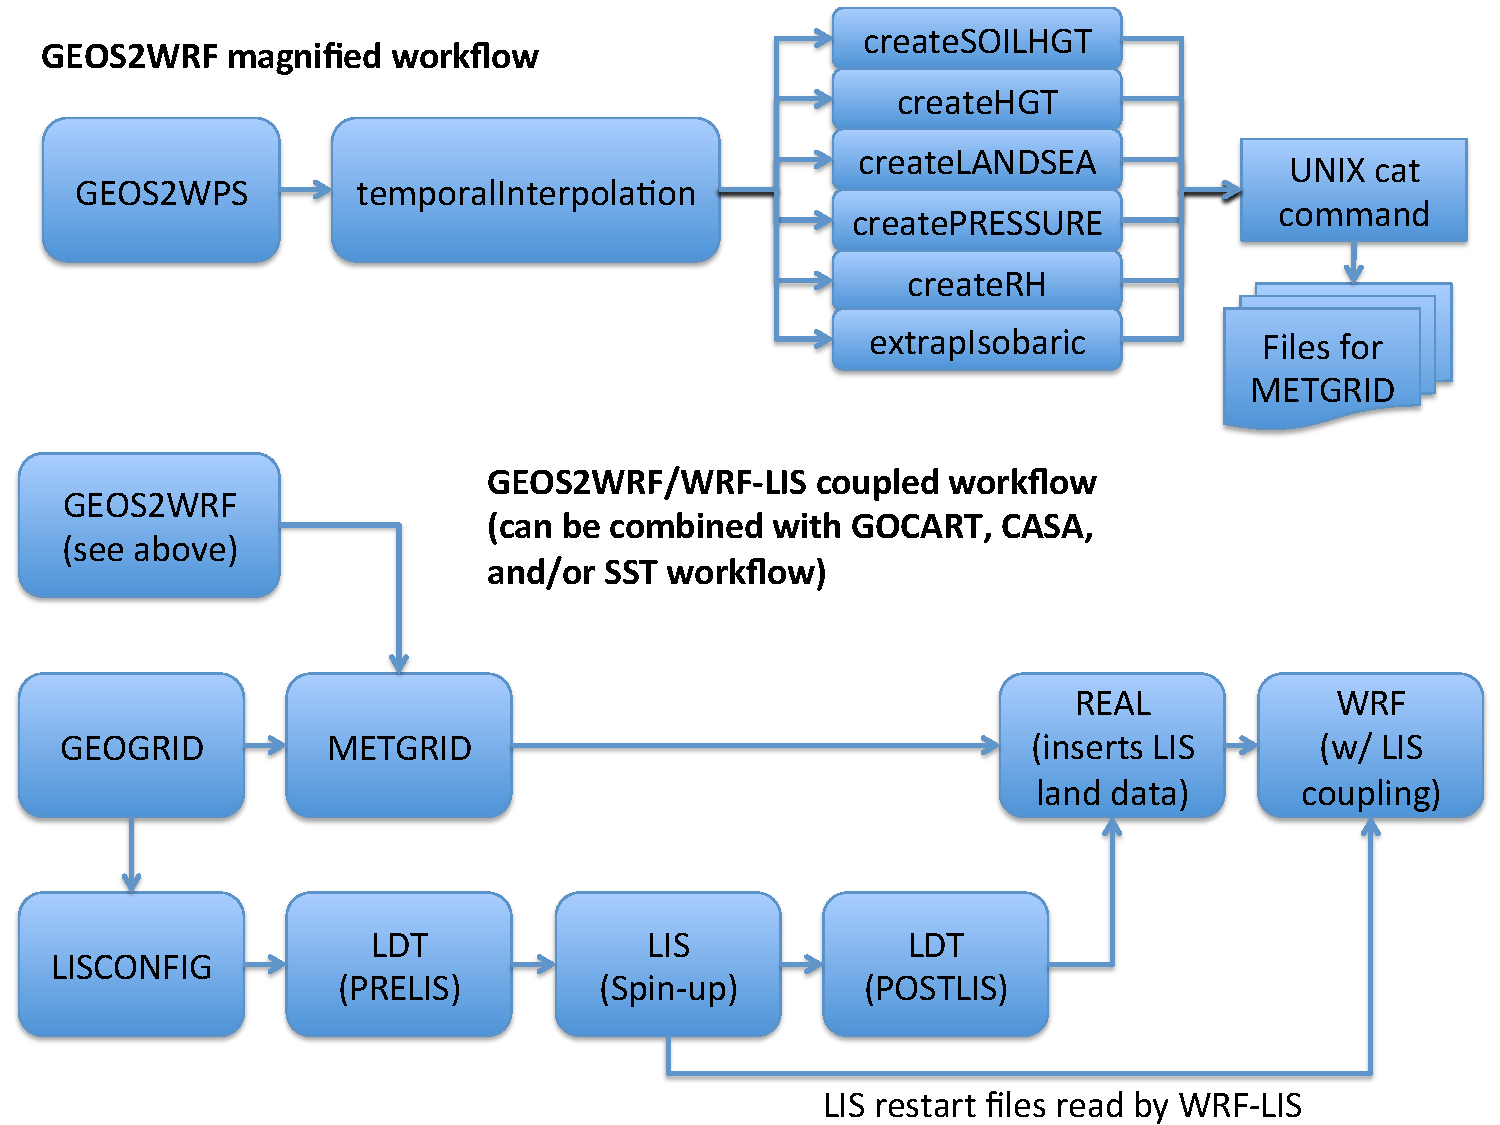
\includegraphics[width=4.5in]{GEOS_workflow}}

A sample script (\texttt{scripts/discover/run\_geos2wrf\_merra2\_3hrassim.sh}) 
is available to use GEOS2WRF to process 3-hourly MERRA-2 assimilation data.
These data are output from GEOS-5 when the global model is adjusting 
toward a MERRA-2 6-hourly analysis via Incremental Analysis Updates [see 
section 4.2 of~\cite{ref:RieneckerEtAl2008}]. This script will run GEOS2WPS,
createLANDSEA, createSOILHGT, and createRH to process the data. To run,
the user must edit the accompanying \texttt{config.discover.sh} file to set the
path to the NU-WRF code, the work directory, and the modules used to
compile GEOS2WRF; then, the \texttt{run\_geos2wrf\_merra2\_3hrassim.sh} should
be modified to specify the start and end dates and hours to process. (Users
who wish to use 6-hourly MERRA or MERRA-2 data can use either GEOS2WRF or
MERRA2WRF; however, the 3-hourly MERRA-2 data can only be processed with 
GEOS2WRF.)

\subsubsection{MERRA2WRF}
\label{subsec:MerraWorkflow}

MERRA2WRF is a monolithic program customized to process the 6-hourly
reanalyses from MERRA and MERRA-2. It was first developed for MERRA under the
assumption that the archived data files (called ``collections'' in GEOS-5
terminology) would be permanent, making it possible to build a single robust
preprocessing tool. Recently support was added for 6-hourly MERRA-2 fields;
however, 3-hourly MERRA-2 processing is not possible due to significant 
differences in the data collections (users must fall back to GEOS2WRF for 
these 3-hourly data).

MERRA and MERRA-2 files are accessible from the NASA GES DISC web page
(\url{http://disc.sci.gsfc.nasa.gov/daac-bin/DataHoldings.pl}), and are 
available to the general public. MERRA-2 files are also accessible on the NASA
Discover supercomputer in\\
\texttt{/discover/nobackup/projects/gmao/merra2/merra2/scratch/}, but are only
available to select users authorized by the GMAO.

MERRA2WRF is compiled when running \texttt{./build.sh geos2wrf}. The following
files must then be gathered from the MERRA or MERRA-2 datasets:

\begin{itemize}
\item \textbf{const\_2d\_asm\_Nx} (in HDFEOS2 or NETCDF format):
  \begin{itemize}
  \item 'XDim'  or 'lon' (longitude)
  \item 'YDim' or 'lat' (latitude)
  \item 'PHIS' (surface geopotential)
  \item 'FRLAKE' (lake fraction)
  \item 'FROCEAN' (ocean fraction)
  \end{itemize}

\item \textbf{inst6\_3d\_ana\_Nv} (variable names are HDF4 or netCDF or 
HDFEOS2):
  \begin{itemize}
  \item 'longitude' or 'XDim'  or 'lon' (longitude)
  \item 'latitude' or 'YDim' or 'lat' (latitude)
  \item 'time' or 'TIME:EOSGRID' or 'TIME' (synoptic hour)
  \item 'levels' or 'Height' or 'lev' (nominal pressure for each model level)
  \item 'ps' or 'PS' (surface pressure)
  \item 'delp' or 'DELP' (layer pressure thicknesses)
  \item 't' or 'T' (layer temperature)
  \item 'u' or 'U' (layer eastward wind)
  \item 'v' or 'V' (layer northward wind)
  \item 'qv' or 'QV' (layer specific humidities)
  \end{itemize}

\item \textbf{inst6\_3d\_ana\_Np} (variable names are HDF4 or netCDF or 
HDFEOS2):
  \begin{itemize}
  \item 'longitude' or 'XDim' or 'lon' (longitude)
  \item 'latitude' or 'YDim' or 'lat' (latitude)
  \item 'time' or 'TIME:EOSGRID' or 'TIME' (synoptic hours)
  \item 'slp' or 'SLP' (sea level pressure)
  \end{itemize}

\item \textbf{tavg1\_2d\_slv\_Nx}  (variable names are HDF4 or netCDF or 
HDFEOS2):
  \begin{itemize}
  \item 'longitude' or 'XDim'  or 'lon' (longitude)
  \item 'latitude' or 'YDim' or 'lat' (latitude)
  \item 'time' or 'TIME:EOSGRID' or 'TIME' (synoptic hours)
  \item 'u10m' or 'U10M' (10-meter eastward wind)
  \item 'v10m' or 'V10M' (10-meter northward wind)
  \item 't2m' or 'T2M' (2-meter temperature)
  \item 'qv2m' or 'QV2M' (2-meter specific humidity)
  \item 'ts' or 'TS' (skin temperature)
  \end{itemize}

\item \textbf{tavg1\_2d\_ocn\_Nx} (variable names are HDF4/netCDF or HDFEOS2):
  \begin{itemize}
  \item 'longitude' or 'XDim' or 'lon' (longitude)
  \item 'latitude' or 'YDim' or 'lat' (latitude)
  \item 'time' or 'TIME:EOSGRID' or 'TIME' (synoptic hours)
  \item 'frseaice' or 'FRSEAICE' (sea ice fraction)
  \end{itemize}

\end{itemize}

Note that the tavg1\_2d\_slv\_Nx and tavg1\_2d\_ocn\_Nx collections are 1-hour 
averages that are valid at the bottom of the hour. For simplicity, MERRA2WRF
uses the 00:30Z average data with the 00Z instantaneous fields, the 06:30Z
average data with the 06Z instantaneous fields, and so on.

The user download the MERRA data and run MERRA2WRF for a specified start date
and end data using the command:
\begin{quote}
  \texttt{./Run\_MERRA.csh StartDate EndDate OutputDir NUWRFDIR}
\end{quote}
A namelist file will be created for each processing date, and files readable 
for METGRID will be generated.  

To use MERRA-2 reanalysis, the user may download MERRA-2 files from the
GES DISC web page and process them with MERRA2WRF by running:
\begin{quote}
\texttt{./proc\_merra2\_ges\_disc.sh StartDate EndDate RunDir NUWRFDIR}
\end{quote}

Alternatively, the user can copy MERRA2 files from the GMAO MERRA2 Discover 
directory and run MERRA2WRF using the command:
\begin{quote}
  \texttt{./Run\_MERRA2.csh StartDate EndDate OutputDir NUWRFDIR}.
\end{quote} 
A namelist file will be created for each processing date, and files readable 
for METGRID will be generated.  

A third alternative is to customize \texttt{namelist.merra2wrf} by hand to 
process the selected MERRA files and \texttt{namelist.merra2\_2wrf} to process
the selected MERRA-2 files. The namelist files consists of a single block:

\begin{tabular}{|l|l|} \hline
Variable Names & Description \\ \hline
\&input          & \\ \hline
outputDirectory  & String, lists directory for writing WPS \\
                 & output files. \\ \hline
merraDirectory   & String, lists directory containing \\
                 & MERRA or MERRA-2 input files. \\ \hline
merraFormat\_const\_2d\_asm\_Nx & Integer, specifies format of\\
 &  const\_2d\_asm\_Nx file. \\ 
 &  1=HDF4, 2=netCDF, 4=HDFEOS2. \\ \hline
merraFile\_const\_2d\_asm\_Nx & String, name of const\_2d\_asm\_Nx file. \\ \hline
numberOfDays & Integer, lists number of days to \\
& process. Each MERRA or MERRA-2 collection. \\
& (excluding const\_2d\_asm\_Nx) will \\
& have one file per day. \\ \hline
merraDates(:) & Array of strings, list each day to be\\
 &  processed (format is YYYY-MM-DD). \\ \hline
merraFormat\_inst6\_3d\_ana\_Nv & Integer, specifies format of\\
 & inst6\_3d\_ana\_Nv files.\\
 &  1=HDF4, 2=netCDF, 4=HDFEOS2. \\ \hline
merraFiles\_inst6\_3d\_ana\_Nv(:) & Array of strings, specifying names of \\
 & inst6\_3d\_ana\_Nv files. \\ \hline
merraFormat\_inst6\_3d\_ana\_Np & Integer, specifies format of\\
 & inst6\_3d\_ana\_Np files. \\
 & 1=HDF4, 2=netCDF, 4=HDFEOS2. \\ \hline
merraFiles\_inst6\_3d\_ana\_Np(:) & Array of strings, specifying names of\\
 & inst6\_3d\_ana\_Np files. \\ \hline
merraFormat\_tavg1\_2d\_slv\_Nx & Integer, specifies format of \\
 & tavg1\_2d\_slv\_Nx files. \\
 & 1=HDF4, 2=netCDF, 4=HDFEOS2. \\ \hline
merraFiles\_tavg1\_2d\_slv\_Nx(:) & Array of strings, specifying names of\\
 & tavg1\_2d\_slv\_Nx files. \\ \hline
merraFormat\_tavg1\_2d\_ocn\_Nx & Integer, specifies format of \\
 & tavg1\_2d\_ocn\_Nx files. \\
 & 1=HDF4, 2=netCDF, 4=HDFEOS2. \\ \hline
merraFiles\_tavg1\_2d\_ocn\_Nx(:) & Array of strings, specifying names of\\
 & tavg1\_2d\_ocn\_Nx files. \\ \hline
\end{tabular}\\

The software is run by typing \texttt{./merra2wrf.x namelist.merra2wrf}. The
output files will be named \texttt{MERRA:\$YYYY-\$MM-\$DD\_\$HH}, where \$YYYY
is the four-digit year, \$MM is the two-digit month, \$DD is the two-digit day,
and \$HH is the two-digit hour. These files are readable by METGRID.  

\centerline{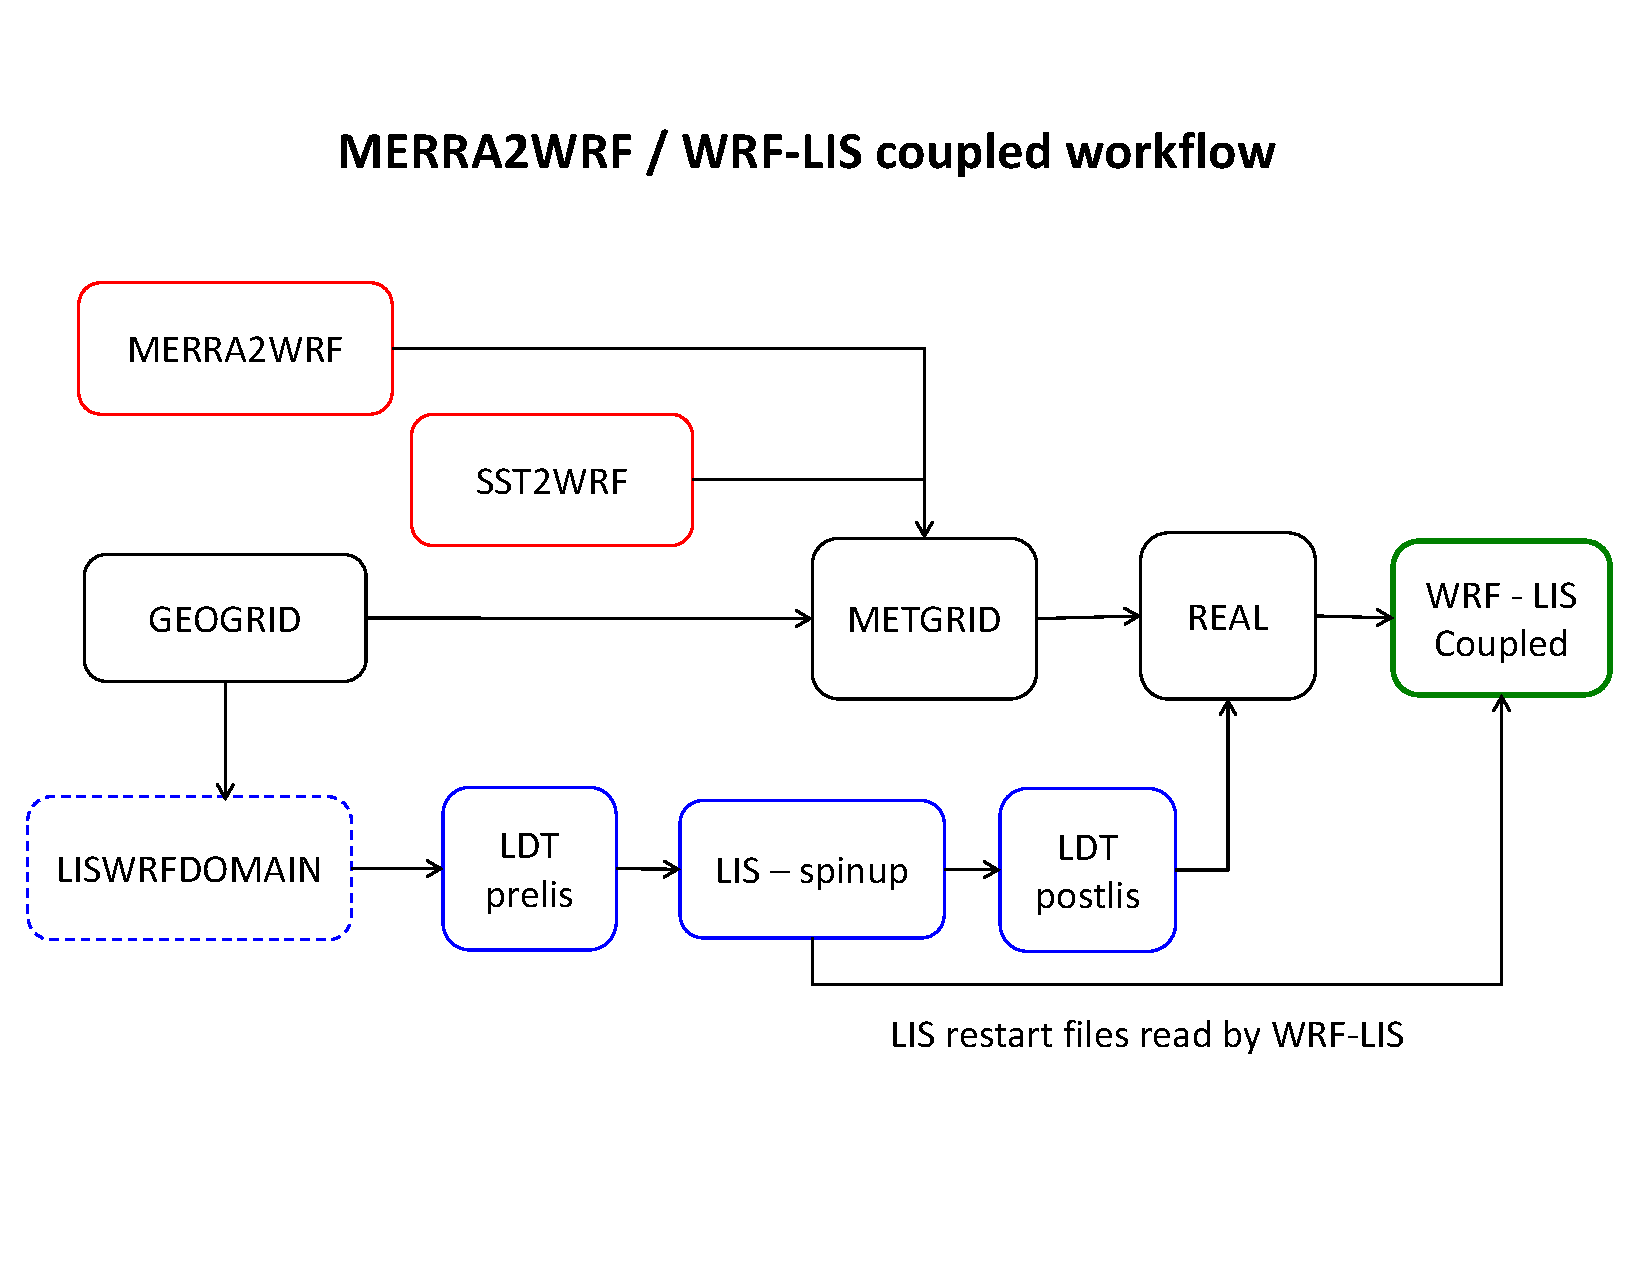
\includegraphics[width=5in]{MERRA_workflow}}

\subsection{Use of New Erodible Soil Options}
\label{subsec:ErodWorkflow}

NU-WRF includes several new options for specifying erodible soil (EROD) for
dust emissions~\citep{ref:ErodUserGuide}. The workflow depends a bit on the 
particular option selected, but requires compilation of WRF-Chem and WPS 
(\texttt{./build.sh chem,wps} if using normal chemistry, or 
\texttt{./build.sh kpp,wps} if using KPP chemistry).

The four available EROD options are:
\begin{itemize}
\item \textbf{EROD\_STATIC}. This is the EROD option inherited from the 
community WRF. Annual EROD at 0.25 deg resolution for sand, silt, and clay is 
processed and fed to WRF-Chem.
\item \textbf{EROD\_MDB}. This is a new seasonal EROD dataset derived from
MODIS-Deep Blue climatological aerosol products. [See 
\cite{ref:GinouxEtAl2012} and \cite{ref:GinouxEtAl2010} for description of
estimating frequency of occurrance of optical depth -- these are converted
to EROD]. Data are subdivided into three groups (for sand, silt, and clay) at 
0.1 deg resolution for four meteorological seasons (December-January-February,
March-April-May, June-July-August, September-October-November). These are 
processed and passed to WRF-Chem. 
\item \textbf{EROD\_DYN\_CLIMO}. This is a new ``dynamic climatological'' EROD
option. It uses a monthly surface bareness field derived at 30 arc second
resolution from the community WRF climatological MODIS vegetation fraction
dataset (\texttt{greenness\_fpar\_modis/}), with adjustments from the 
community WRF's soil type and MODIS and USGS land use datasets to screen out 
water bodies. It also uses a 30 arc second topographic depression dataset 
derived from the community WRF's terrain dataset. These fields are passed to 
WRF-Chem, which will create an instantaneous EROD field from these variables 
with adjustments to screen out snowy or very cold locations.
\item \textbf{EROD\_DYN}. This is a new ``dynamical'' EROD option. It uses
the same topographic depression field as \textbf{EROD\_DYN\_CLIMO}, plus
a surface bareness field based on either NASA GIMMS or NASA SPoRT daily NDVI
products.  The data are passed to WRF-Chem, which will construct an 
instantaneous EROD field from the bareness and topographic depression with 
adjustments to screen out snowy or very cold locations. 
\end{itemize}

A sample workflow for EROD is presented here:
\begin{itemize}
\item \textbf{Assemble GEOG data}. Several new EROD-related fields must be
obtained from the NU-WRF group and placed in subdirectories with the standard
GEOG data available with the community WRF. For \textbf{EROD\_MDB}, they are
\texttt{erod\_mdb\_clay\_0.1deg/}, \texttt{erod\_mdb\_sand\_0.1deg/}, and\\
\texttt{erod\_mdb\_silt\_0.1deg/}. For \textbf{EROD\_DYN\_CLIMO}, they are\\
\texttt{bareness\_dyn\_climo/} and \texttt{TOPODEP\_30s/}. For
\textbf{EROD\_DYN}, the \texttt{TOPODEP\_30s/} data must be staged; in 
addition, the user is advised to collect NDVI-based greenness in GEOGRID 
format from NASA SPoRT and place the files in a \texttt{gvfsport/} directory.

\item \textbf{Create NDVI-based bareness for EROD\_DYN option}. The 
NDVIBARENESS4WRF tool is used to process NDVI data and generate a bareness
field.  Both bareness and NDVI are written in WPS intermediate format for
direct ingest into METGRID.  The NDVIBARENESS4WRF code is described by
\cite{ref:NdviBareness4WrfUserGuide}.

\item \textbf{GEOGRID}. Run for terrestrial processing. Use the 
\texttt{GEOGRID.TBL.ARW\_CHEM\_NUWRF} file to ensure EROD related fields
are specified. If preparing for the \textbf{EROD\_DYN} option, ``gvfsport'' 
should be specified as the first part of the ``geog\_data\_res'' option in 
\texttt{namelist.wps} -- this will ensure the SPoRT greenness is processed
rather than the climatological greenness data available with the community
WRF.

\item \textbf{UNGRIB}. Run for normal GRIB file processing.

\item \textbf{METGRID}. Run for normal processing. If preparing for the
\textbf{EROD\_DYN} option, user should modify \texttt{namelist.wps} to 
include the file prefix(es) for the bareness data in the 
``fg\_name'' namelist option. Note that the \texttt{METGRID.TBL.ARW} file
in NU-WRF has been modified to recognize the new EROD-related fields.

\item \textbf{REAL}. Run to produce initial and lateral boundary conditions.
Namelist variable ``chem\_opt'' should be set to 401 for simple dust 
treatment. (Dust emissions can also be used with GOCART chemistry
by setting ``chem\_opt'' to 300, 301, 302, or 303; however, in this case
the workflow must be expanded to include the steps in 
Section~\ref{subsec:GocartWorkflow}.) New namelist variable ``erod\_option'' 
in the \&chem block should be set to ``static'', ``mdb'', ``dyn\_climo'', or 
``dyn''. If not set, ``static'' is assumed.

\item \textbf{WRF}. Run for EROD simulation. Optionally set the new
``gocart\_dustemiss\_layer'' namelist variable to highest vertical model level
to spread dynamic dust (default is 1), or set 
``gocart\_dustemiss\_suppress=1'' to shut off dynamic dust emissions. The new 
variable EROD\_TIMESTEP in the wrfout netCDF file will show the instantaneous 
EROD field for sand, silt, and clay for whatever EROD option is used. Other 
variables of note are:

\begin{itemize}
\item BARENESS\_DYN\_CLIMO: Monthly input bareness field for\\
  \textbf{EROD\_DYN\_CLIMO} option.
\item EROD\_MDB\_CLAY: Seasonal EROD for clay for \textbf{EROD\_MDB} option.
\item EROD\_MDB\_SAND: Seasonal EROD for sand for \textbf{EROD\_MDB} option.
\item EROD\_MDB\_SILT: Seasonal EROD for silt for \textbf{EROD\_MDB} option.
\item EROD\_STATIC: The standard EROD field available with the community WRF.
\item TOPODEP: The topographic depression values for sand, silt, and clay
for the \textbf{EROD\_DYN\_CLIMO} and \textbf{EROD\_DYN} options.
\end{itemize}

\end{itemize}

\subsection{Use of GOCART Aerosol Data}
\label{subsec:GocartWorkflow}

NU-WRF offers advanced aerosol modeling using the implementation of GOCART
 [see \cite{ref:ChinEtAl2002} and \cite{ref:GinouxEtAl2001}] in WRF-Chem. 
Running GOCART in WRF allows for aerosol coupling with the Goddard 3ICE and 
4ICE microphysics schemes and with the 2011, 2014 or 2017 Goddard radiation 
schemes, providing simulation of the direct and indirect aerosol effects on 
weather and climate. For best results, it is necessary to provide initial and 
lateral boundary conditions for GOCART, plus surface based emissions. To that 
end, the NU-WRF modeling system includes the new GOCART2WRF preprocessor for 
providing chemical boundary conditions from the GEOS-5, and includes the 
community PREP\_CHEM\_SOURCES program for emissions. To run, the user must 
compile with
\texttt{./build.sh chem,wps,gocart2wrf,prep\_chem\_sources,plot\_chem}.

GOCART2WRF supports four possible sources of GOCART data: 

\begin{itemize}

\item offline GOCART;

\item on-line GOCART from GEOS-5;

\item MERRAero reanalyses~\citep{ref:KishchaEtAl2014}; and

\item MERRA-2~\citep{ref:BosilovichEtAl2015} reanalyses.  

\end{itemize}

A workflow supporting the use of GOCART in NU-WRF might look like this:

\begin{itemize}
\item \textbf{WPS}. Perform terrestrial and meteorological preprocessing as 
normal.
\item \textbf{REAL}. Generate meteorological initial and lateral boundary
conditions as normal.
\item \textbf{GOCART2WRF}. Process GOCART data and insert into output
files from REAL. Typically the user must edit a \texttt{namelist.gocart2wrf} 
to specify the number of WRF domains, location of REAL output files, and 
location, source, and file prefixes of the GOCART files. GOCART2WRF is then 
executed at the command line using \texttt{./gocart2wrf} with 
\texttt{namelist.gocart2wrf} in the current working directory. GOCART2WRF will
obtain the required dates and times from the REAL netCDF files, search the 
GOCART files for the corresponding dates and times, read and interpolate
the required GOCART variables, and essentially append those fields to the
REAL files. Currently 17 GOCART variables are processed: Hydrophobic and 
Hydrophilic Black Carbon, Hydrophobic and Hydrophilic Organic Carbon, dust 
particles with 0.5 $\mu$m, 1.4 $\mu$m, 2.4 $\mu$m, 4.5 $\mu$m, and 8.0 $\mu$m 
effective radii, sea salt particles with 0.3 $\mu$m, 1.0 $\mu$m, 3.2 $\mu$m, 
and 7.5 $\mu$m effective radii, and concentrations of Dimethyl Sulfide, 
Methanesulfonic Acid, Sulfur Dioxide, and Sulfate.

The \texttt{namelist.gocart2wrf} file contains the following entries:

\begin{tabular}{|l|l|} \hline
Variable Names & Description \\ \hline
\&wrf          & \\ \hline
max\_dom & Integer, specifies number of WRF domains. \\ \hline
wrf\_dir & String, specifies directory with wrfinput \\ 
         &  and wrfbdy files. \\ \hline
\&gocart\_shared & \\ \hline
gocart\_format & Integer, specifies format of GOCART data; \\ 
               & currently must be set to 5 (for netCDF4 files) \\ \hline
gocart\_source & String, lists source of GOCART data. \\
               & 4 options are available: \\
               & 'GEOS'     : Output from GEOS-5 (default) \\
               & 'MERRA2'   : Output from MERRA-2 reanalysis \\
               & 'MERRAERO' : Output from MERRAero reanalysis \\
               & 'OFFLINE'  : Output from offline GOCART \\ \hline
gocart\_dir & String, specifies directory with netCDF4 GOCART \\
            & files to process.  If processing MERRAero or MERRA2 data, \\
            & files are assumed to be in subdirectories, e.g., \\
            & For MERRAERO: \texttt{gocart\_dir/Y2005/M05/} \\
            & For MERRA-2:  \texttt{gocart\_dir/\$STREAM/stage/Y2005/M05/} \\
            &  where \$STREAM is MERRA2\_100 for data before 1992, \\
            &  MERRA2\_200 for data from 1992 to 2000, \\ 
            &  MERRA3\_300 for data from 2001 to 2010, or \\
            &  MERRA2\_400 for data from 2011 on. \\
gocart\_prefix & String, specifies file name prefix for netCDF4 GOCART \\
               & files. Ignored if processing MERRA-2 or MERRAero data.\\ \hline
\end{tabular} \\

If processing MERRA-2 data, the user can download MERRA-2 GOCART files from
the GES DISC web page, and process them with GOCART2WRF.  The command is:
\begin{quote}
  \texttt{./proc\_merra2\_gocart\_ges\_disc.sh NumDomains StartDate EndDate RunDir NUWRFDIR}
\end{quote}
A namelist file will be created by the script, and updated 
\texttt{wrfbdy\_d01} and \texttt{wrfinput\_d*} netCDF files will be created.

\item \textbf{PREP\_CHEM\_SOURCES}. This community tool processes a number of
biogenic, anthropogenic, volcanic, and wildfire 
emissions~\citep{ref:FreitasEtAl2011}. Operating this program is largely 
described in \cite{ref:WrfChemEmissionsGuide} and \cite{ref:WrfChemUserGuide},
and requires customizing a \\
\texttt{prep\_chem\_sources.inp} file and downloading emissions data supported
by the program. The NU-WRF version has several modifications:

\begin{itemize}

\item \textbf{Map projection}. The map projection code from WPS has been added
to PREP\_CHEM\_SOURCES to ensure consistency in emission interpolation. This
support is automatic when using the NU-WRF build system, and no user action
is required.

\item \textbf{Improved GOCART background fields}. Processing emissions for
GOCART requires monthly climatological background fields of 
Hydrogen Peroxide, Hydroxide, and Nitrate. The community data for
PREP\_CHEM\_SOURCES contains 55 vertical levels, is only for 2006, and is 
missing some information useful for vertical interpolation. New 72-level
datasets produced by GSFC are now available in two formats with improved 
vertical interpolation information.  The user should edit
\texttt{prep\_chem\_sources.inp} and set the new 
``gocart\_bg\_data\_type'' variable to ``old'' or ``new'' to switch between the
community and new files. If ``new'' files are selected, they must be in a
\texttt{gocart\_bg\_new/} subdirectory on the same level as the 
\texttt{gocart\_bg/} folder containing the community 55-level files. If 
``new'' is selected, the program will first search for 
\texttt{geos5\_met\_1MAVG\_YYYYMM.nc} and 
\texttt{gmi\_merra\_oxidants\_YYYYMM\_1.25x1.nc} files, where YYYY is the 
4-digit year and MM is the 2-digit month. If the program fails to find both 
files, it will fall back on \texttt{gmi\_2006MM.nc} files, which are also new
72-level files but only exist for 2006.

\item \textbf{Improved interpolation of GOCART background fields}. The
community PREP\_CHEM\_SOURCES program uses simple averaging of GOCART
background grid points to each WRF grid point, which implicitly assumes the
WRF grid is at a coarser resolution than the background. This results in
unphysical blocky fields, which are further marred by gradients associated
with sharp WRF terrain. In the NU-WRF version of PREP\_CHEM\_SOURCES, 
bilinear interpolation is used in cases where less than two background grid
points are averaged to a WRF grid point, leading to much smoother fields.

\item \textbf{GFEDv4}. The GFEDv4 biomass burning emissions dataset
[\cite{ref:RandersonEtAl2015}] is supported. It supersedes and replaces the Global Fire Emissions Database, Version 3.1 (GFEDv3.1). To use it the user must edit the \texttt{prep\_chem\_sources.inp} file, toggle the new  variable ``use\_gfedv4=1'', set the new ``gfedv4\_data\_dir'' variable to 
specify the directory with the GFEDv4 data, and edit the new 
``gfedv4\_suffix'' variable to list the species to process.  
There are sample \texttt{prep\_chem\_sources.inp} files
in the scripts/regression/testcases/chem directories with default settings
for the DISCOVER system. Note that GFEDv4 and other GFED data sets cannot be used 
simultaneously. Currently the following species can be processed: BC, C2H4, C2H4O, C2H4, C2H5OH, C2H6S, C2H6, C3H6O, C3H6, C3H8, CH4, C5H8, CH2O, CH3OH, CH4, CO2, CO, NH3, NOx, OC, 
PM2p5, SO2, Terpenes, Toluene\_lump, and TPM. DM can also be processed but is 
not currently used by WRF-Chem.

\item \textbf{QFED}. The NASA QFED wildfire emissions dataset 
[\cite{ref:QfedDocumentation}] is supported. The user must edit the 
\texttt{prep\_chem\_sources.inp} file, toggle the new variable ``use\_qfed=1'',
set the new ``qfed\_data\_dir'' variable to specify the top directory with QFED
data (yearly subdirectories like \texttt{Y2005/} are assumed, with monthly 
subdirectories like \texttt{M05/} within each annual subdirectory), and edit 
the new ``qfed\_suffix'' variable to list the species to process (e.g, 
``bc,oc,pm25,so2''). Note that the species are used to construct the names of 
the emissions files (e.g, \texttt{qfed2.emis\_bc.005.20140404.nc4}, so the 
names are case sensitive. Also, note that QFED cannot be used simultaneously 
with GFED source options. Currently the following QFED species can be 
processed: acet, ald2, alk4, bc, c2h6, c3h6, c3h8, ch2o, ch4, co, co2, mek, 
nh3, no, oc, pm25, and so2.

\item \textbf{Output of map projection data}. New \texttt{.map} files with map
projection data are automatically output. These files are 
intended for use by PLOT\_CHEM to visualize the fields. 
\end{itemize}

\item \textbf{PLOT\_CHEM}. This is an optional step to create simple
visualizations of emissions output from PREP\_CHEM\_SOURCES. The program
reads in a GrADS control file produced by PREP\_CHEM\_SOURCES, the 
corresponding GrADS binary file, and the special \texttt{.map} file with 
critical map projection information. PLOT\_CHEM will then create 
visualizations of each field using NCAR Graphics. The plots are not 
publication quality and are only intended for sanity checking. To run, the 
user must first create a symbolic link \texttt{grads.ctl} to the desired 
GrADS control file, and then run \texttt{./plot\_chem} in the same directory 
as the GrADS and \texttt{.map} files. The output is a \texttt{gmeta} file 
which can be viewed using the NCAR Graphics \texttt{idt} program (see 
\url{http://ngwww.ucar.edu} for information on NCAR Graphics).

\item \textbf{CONVERT\_EMISS}. This is a community WRF-Chem preprocessor
that takes the output from PREP\_CHEM\_SOURCES and rewrites the fields in
new netCDF files for reading by WRF-Chem. This program is described in
\cite{ref:WrfChemUserGuide} and \cite{ref:WrfChemEmissionsGuide}, and requires
modifying a \texttt{namelist.input} file to specify domain information, 
physics, and chemistry options.  The program is then run in the same directory
as the \texttt{namelist.input} and the PREP\_CHEM\_SOURCES output files.

There are two issues to keep in mind:
\begin{itemize}
\item First, CONVERT\_EMISS does not currently process more than one domain at
  a time. Thus, the user must process each domain in separate executions, and 
  must rename the input files to use ``d01'' before execution, regardless of 
  what the actual domain number is. The output files must then be renamed to 
  restore the actual domain numbers for WRF-Chem. In addition, a 
  \texttt{namelist.input} file must be customized for each execution with the 
  ``max\_dom'' variable set to ``1'' and the first grid domain variables
  (e.g., ``dx'', ``nx'', etc) conforming to whichever domain is being 
  processed.
\item Second, the output files from PREP\_CHEM\_SOURCES must be renamed to
  conform to the naming convention expected by CONVERT\_EMISS. The naming
  convention for the different emissions files are documented in 
  \cite{ref:WrfChemEmissionsGuide}.
\end{itemize}

%The NU-WRF version of CONVERT\_EMISS includes support for most GFEDv4.1 and 
%QFED species without any special action required by the user. However, if the 
%user processes C2H4, CH4, CO2, terpenes, or DM emissions from GFEDv3.1 with 
%PREP\_CHEM\_SOURCES -- or ch4 or co2 from QFED -- then the new 
%\texttt{namelist.input} variable ``gfedv3\_biomass\_burn\_extravars'' in the 
%\&chem block must be set to 1. This will cause CONVERT\_EMISS to read the 
%additional fields at the end of the \texttt{emissfire} binary file (these are 
%not produced by the community version of PREP\_CHEM\_SOURCES, so reads are not
%attempted by default to preserve backward compatibility).

Note that if PREP\_CHEM\_SOURCES processed ``new'' GOCART background files,
the \&chem block in \texttt{namelist.input} must be modified to add
``new\_gocart\_bg\_files=.true.'' so CONVERT\_EMISS will read 72 levels
of data and perform correct vertical interpolation.  If this setting is 
omitted, the background fields output by CONVERT\_EMISS will likely contain 
unphysical values.

\item \textbf{WRF-Chem}. Running WRF-Chem is similar to the basic case in 
section~\ref{subsec:BasicWorkflow}, but requires the \&chem namelist block
to be included in the \texttt{namelist.input} with with GOCART activated
(chem\_opt = 300, 301, 302, or 303). Aerosol coupling with the Goddard
3ICE or 4ICE schemes (mp\_physics=55 or 56) will be activated if the new
``gsfcgce\_gocart\_coupling'' namelist variable is set to 1 (set by 
default). Likewise, aerosol coupling with the 2011, 2014 or 2017 Goddard radiation 
schemes (ra\_lw\_physics=55, 56 or 57 and ra\_sw\_physics=55, 56 or 57) will 
be activated if the new ``gsfcrad\_gocart\_coupling'' namelist variable is set
to 1 (set by default).
\end{itemize}

\centerline{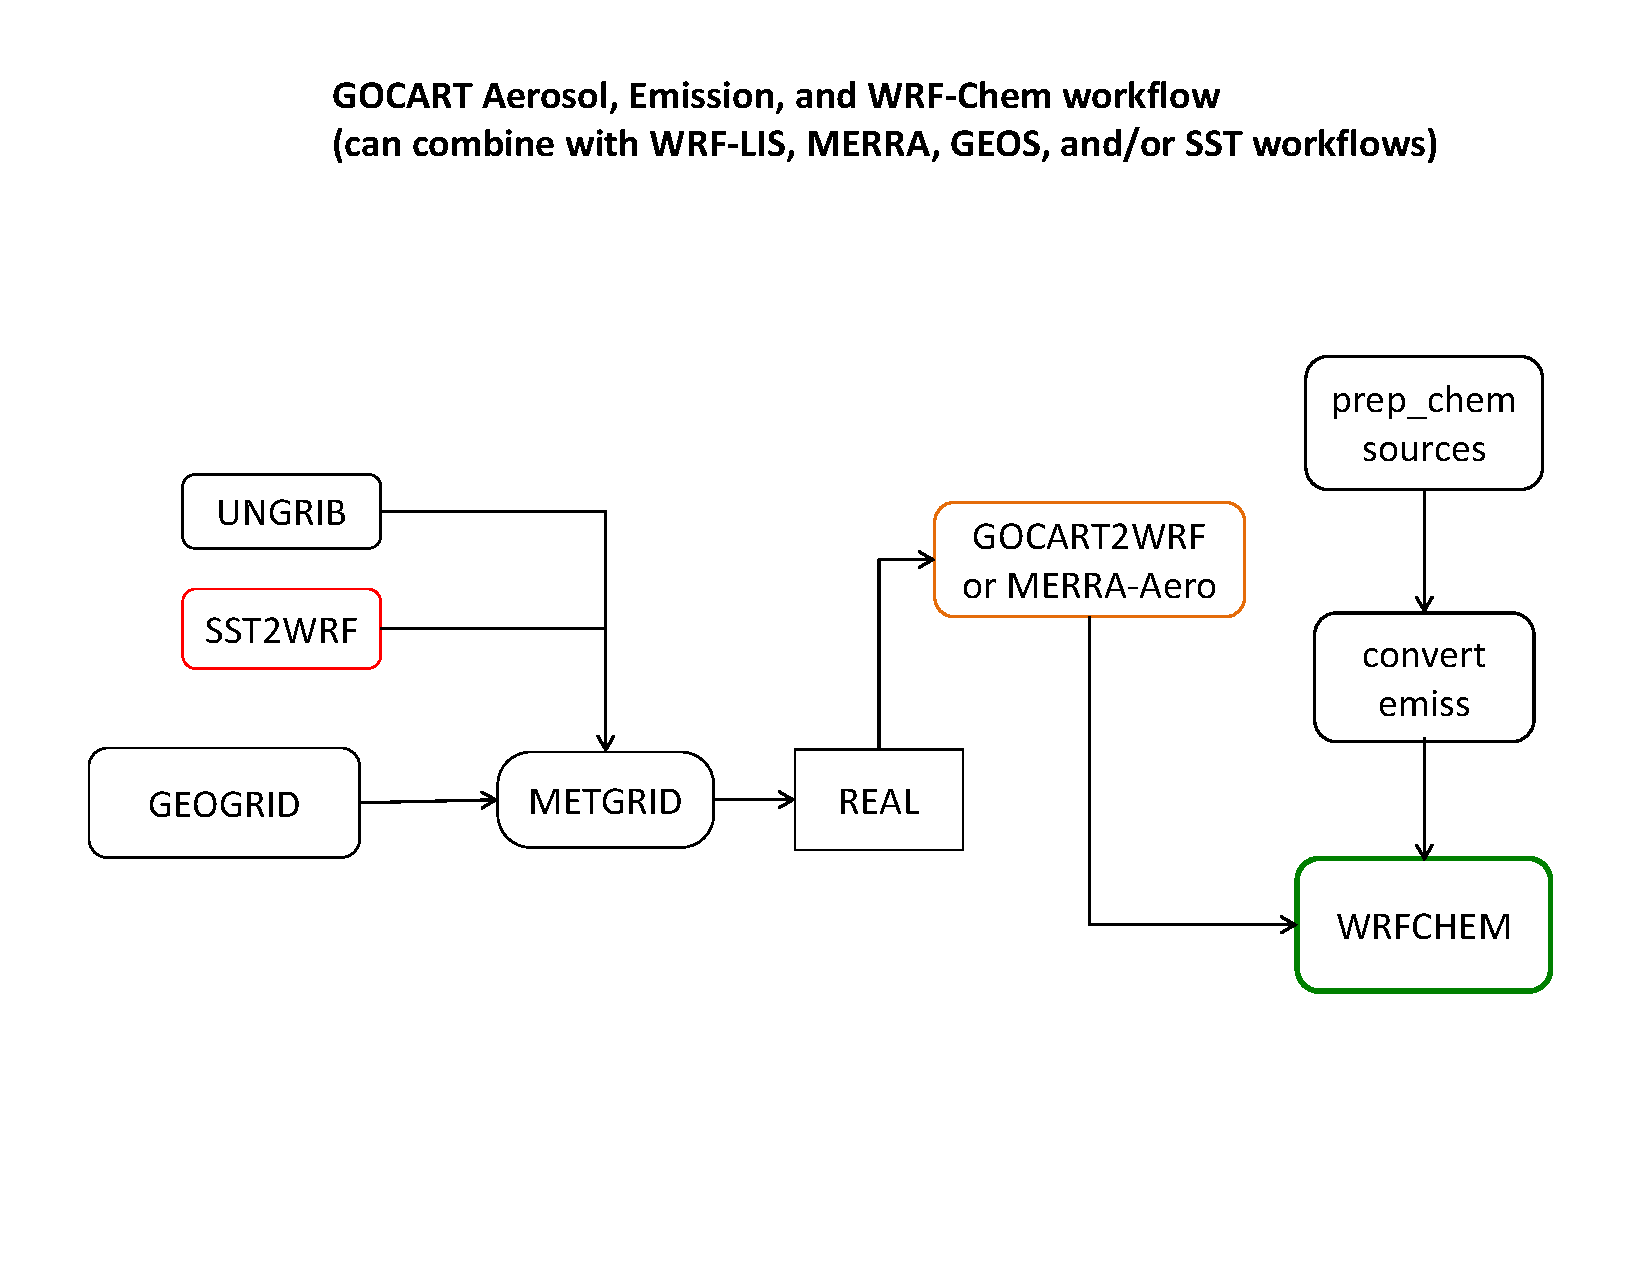
\includegraphics[width=5.5in]{GOCART_emiss_workflow}}

\subsection{Use of CASA CO$_2$ Data}
\label{subsec:CasaWorkflow}

NU-WRF has the capability for running simulations with CO$_2$ treated as
a tracer (i.e., no interaction with physics). This requires specifying initial,
lateral boundary, and flux emission fields of CO$_2$. To that end, several
utilities have been written to process CASA global climatological CO$_2$ 
concentrations and flux emissions and provide them to WRF-Chem: 
READ\_CO2\_CONC, READ\_CO2\_FLUX, and CASA2WRF. 

A particular capability of the CASA2WRF utility allows for the temporal interpolation 
of CASACO2 flux depending on the NU-WRF model state. This capability can
be turned on by modifying the namelist.casa2wrf file and setting  the ``flux\_interpolate'' 
namelist variable equal to 1. With this option, the NU-WRF model state is read by 
CASA2WRF every hour and wrf-domain interpolated CO$_2$ flux components from 6 different sources
\begin{itemize}
\item Respiratory (monthly)
\item Net Production (monthly)
\item Bio-fuel (monthly)
\item Fossil Fuel (yearly)
\item Wild fire (daily) 
\item Ocean CO$_2$
\end{itemize}

are combined to produce total flux and flux tendency netCDF files that can be 
input to NU-WRF WRF-Chem runs. 

To compile, the user must type \texttt{./build.sh casa2wrf}. It creates the 
following executables in \texttt{utils/bin}:

\begin{itemize}

\item \texttt{Read\_CO2\_conc.x}: Reads and converts a CO$_2$ 
  \textbf{concentration} data file to netCDF format usable by NU-WRF.

\item \texttt{Read\_CO2\_Flux.x}: Reads and converts a CO$_2$ 
  \textbf{flux} data file to netCDF format usable by NU-WRF.
  
\item \texttt{ConvertData2Netcdf.x}: Converts CO$_2$ flux 
  component files in binary format to netCDF format.
  
\item \texttt{casa2wrf.x}: Processes and incorporates the CO$_2$ concentration and flux data
  to \texttt{wrfinput\_d*}, \texttt{wrfbdy\_d01}, and flux input files suitable for 
  WRF-Chem runs. 

\end{itemize}

Instructions for running these programs, including namelist definitions,
are provided in \cite{ref:Casa2WrfUserGuide}. A sample workflow is provided 
below:

\begin{itemize}

\item \textbf{WPS}. Perform terrestrial and meteorological preprocessing
  as normal.

\item \textbf{REAL}. Generate meteorological initial and lateral boundary 
  conditions as normal.

\item \textbf{READ\_CO2\_CONC}. Reads the CASA CO$_2$ concentration files in 
  flat binary format, and converts to netCDF with a time stamp. 

\item \textbf{READ\_CO2\_FLUX}. Reads the CASA CO$_2$ flux files in 
  flat binary format, and converts to netCDF with a time stamp. 
  
\item \textbf{ConvertData2Netcdf}. Reads the CASA CO$_2$ flux files from 
  different sources in flat binary format, and converts to netCDF with a time 
  stamp. 
  
\item \textbf{CASA2WRF}. Read the CO$_2$ netCDF files, interpolates 
  concentration and flux data to the WRF grids (single or nested), read the 
  \texttt{wrfout*} files from a NU-WRF run every hour or any specified time 
  interval from namelist, temporally interpolate the NPP and RESP CO$_2$ 
  fluxes with relation the NU-WRF state, combine the fluxes from all sources, 
  calculates the rates of change of flux/hour at the user specified time 
  frequency, appends the interpolated concentrations to the initial and 
  lateral boundary condition netCDF files (\texttt{wrfinput\_*} and 
  \texttt{wrfbdy\_d01}), and writes the interpolated fluxes to a new netCDF 
  file (\texttt{CO2\_domain\_date}).

\item \textbf{WRF-Chem}. Run WRF-Chem with CASA CO$_2$ chemistry options in the
  \texttt{namelist.input} (including chem\_opt = 18, emiss\_opt=18, and 
  emiss\_inpt\_opt=18). Other appropriate settings are listed in
  \cite{ref:Casa2WrfUserGuide}.

\end{itemize}

\centerline{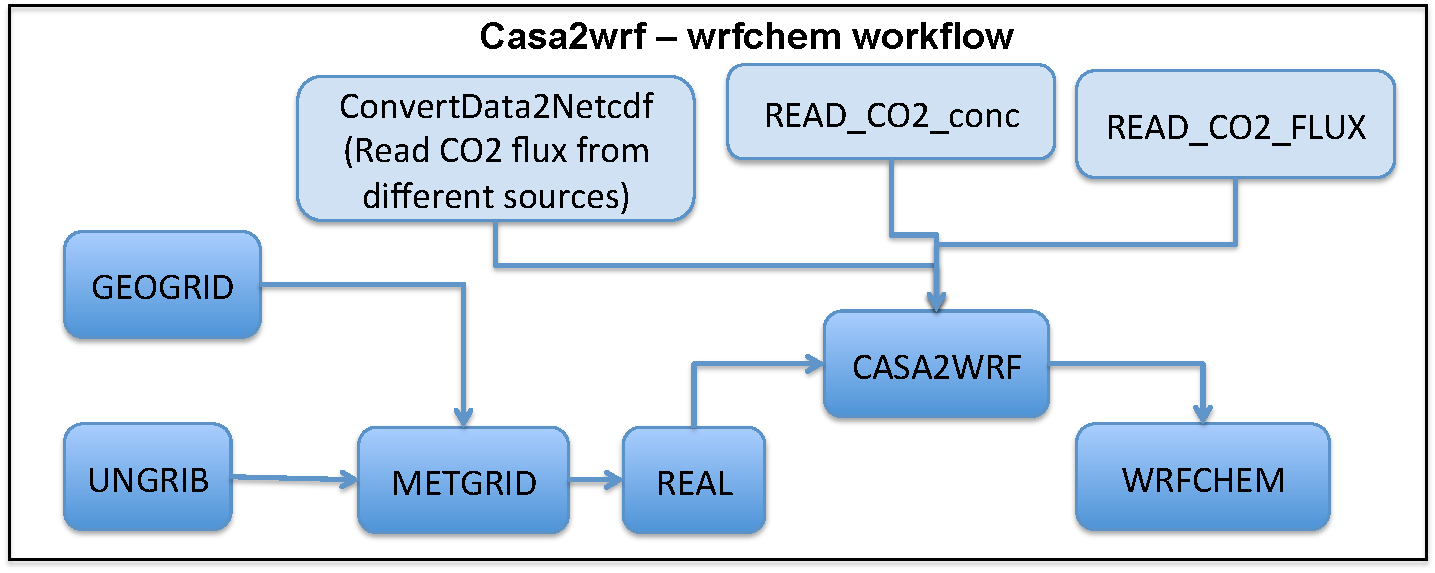
\includegraphics[width=4.75in]{CASA_Flux}}

\subsection{Use of SPoRT Sea Surface Temperature Data}
\label{subsec:SportSST}

NASA SPoRT generates sea surface temperature analyses for the northern 
western hemisphere every 12 hours valid at 06Z and 18Z.  A script\\
\texttt{fetch\_sport\_sst\_northwestHemi.py} is available to download
GRIB2 files of these analyses from the SPoRT FTP site.  The script and
companion configuration file \texttt{sport\_sst\_northwestHemi.cfg} are in the 
\texttt{scripts/python/fetch\_data/} directory.  The configuration file specifies the
start and end dates and hours for downloading data, along with the top 
directory for storing the downloaded files.  The user can override the 
date/time information in this file by running 
\texttt{fetch\_sport\_sst\_northwestHemi.py} with a \texttt{-L} flag (or 
equivalently, \texttt{-{}-latest}) on the command line; this will cause the 
script to fetch all available files valid for the most recent 24 hours.  Files
will be uncompressed via gunzip after being downloaded.

The uncompressed GRIB2 files can be processed by UNGRIB (we recommend using 
the prefix ``SPORT\_SST'' for the output files).  The user must then edit the 
\texttt{namelist.wps} file to include the SPoRT SST prefix in the 
``fg\_name'' namelist variable so METGRID processes the data along with other 
atmospheric fields. When run, METGRID will replace the SST or skin temperature
from atmospheric fields with that from the SPoRT analysis.  The remaining 
steps (REAL and WRF) can be completed as normal.
 
\subsection{Use of RSS Sea Surface Temperature Data}
\label{subsec:RSSSST}

A special preprocessor included with NU-WRF is SST2WRF, which processes
several sea surface temperature (SST) products produced by Remote Sensing
Systems (RSS; see \url{http://www.remss.com}). These products are potential 
alternatives to the SST or skin temperature fields often provided in 
meteorological GRIB files (e.g., from the NOAA GFS or NAM models). Because 
RSS products are not available in GRIB format, UNGRIB cannot process them
and a tool like SST2WRF is required as a substitute.

SST2WRF currently supports several different analysis products classified by 
source instrument and by algorithm version. The instrument SST analyses are
\begin{itemize}
\item \textbf{mw\_ir}. 9-km global SST valid at 1200 UTC based on microwave 
  (TMI, AMSR-E, AMSR2, WindSat) and Infrared (Terra MODIS, Aqua MODIS) data.
\item \textbf{mw}. 25-km global SST valid at 0800 LT, based on Microwave (TMI,
  AMSR-E, AMSR2, WindSat) data.
\end{itemize}

The algorithm versions are:
\begin{itemize}
\item \textbf{rt}. The real-time algorithm.
\item \textbf{v04.0}. Version 4 algorithm.
\end{itemize}

See \url{http://www.remss.com/measurements/sea-surface-temperature/oisst-description} for a description of these products.

A workflow for SST2WRF could be similar to that in section 
\ref{subsec:BasicWorkflow}, but would require running SST2WRF \emph{in 
addition to} UNGRIB. UNGRIB is responsible for processing meteorological 
fields, while SST2WRF will process only the SST related fields from RSS. (One 
could also replace UNGRIB with GEOS2WRF or MERRA2WRF; for simplicity, we will
assume UNGRIB is used.)

The user must compile using \texttt{./build.sh sst2wrf}. A script given in \\
\texttt{scripts/discover/fetch\_rss\_sst.sh} can be used to download SST data. First,
edit fetch\_rss\_sst.ss and set the variables NUWRFDIR
and WORKDIR. Then run by typing \texttt{fetch\_rss\_sst.sh startdate enddate instrument\_type}.
The retrieved files can then be processed using the batch script at\\ 
\texttt{scripts/discover/run\_sst2wrf.discover.sh}. As an alternative, the
user can customize a sample namelist file given in \\
\texttt{utils/sst2wrf/namelist/namelist.sst2wrf} to provide the 
following information:\\

\begin{tabular}{|l|l|} \hline
Variable Names & Description \\ \hline
\&input          & \\ \hline
instrument & String, specifies instrument(s) used for analysis; \\ 
           & options are ``mw\_ir'', ``mw''. \\  \hline
year & Integer, specifies valid year of analysis. \\ \hline
dayOfYear & Integer, specifies valid day of year of analysis. \\ \hline
version & String, specifies algorithm for analysis; \\
        & options are ``rt'',''v04.0''. \\ \hline
inputDirectory & String, specifies directory with SST file. \\ \hline
\&output & \\ \hline
outputDirectory & String, specifies directory for output file. \\ \hline
prefixWPS & String, specifies file name prefix for output; \\ 
          & prefix must also be in \texttt{METGRID.TBL} for \\
          & METGRID to process. \\ \hline
\&fakeoutput & \\ \hline
numFakeHours & Integer, specifies number of hours of each day \\ 
             & that additional WPS files should be written for. \\
             & Currently only one SST analysis is available \\
             & per day, but METGRID requires all time varying \\
             & fields to have same time interval. Thus, we \\
             & optionally output daily SST at multiple times \\
             & corresponding to when atmospheric data are \\
             & available. \\ \hline
fakeHours & Array of integers, specifies nominal hours of day \\
          & in UTC for an input daily SST analysis to be \\
          & output. \\ \hline
\end{tabular} \\

The program is then run by typing \texttt{./sst2wrf} in the same directory
as \texttt{namelist.sst2wrf}. 

The resulting output files will be in WPS intermediate format. The user must 
then edit \texttt{namelist.wps} and list both the meteorological (from UNGRIB)
and SST (from SST2WRF) file prefixes in the ``fg\_name'' namelist variable 
[see Chapter 3 of \cite{ref:ArwUserGuide}]. METGRID will replace the SST
or skin temperature from UNGRIB with that from SST2WRF. The remaining
steps (REAL and WRF) can be completed as normal.

\centerline{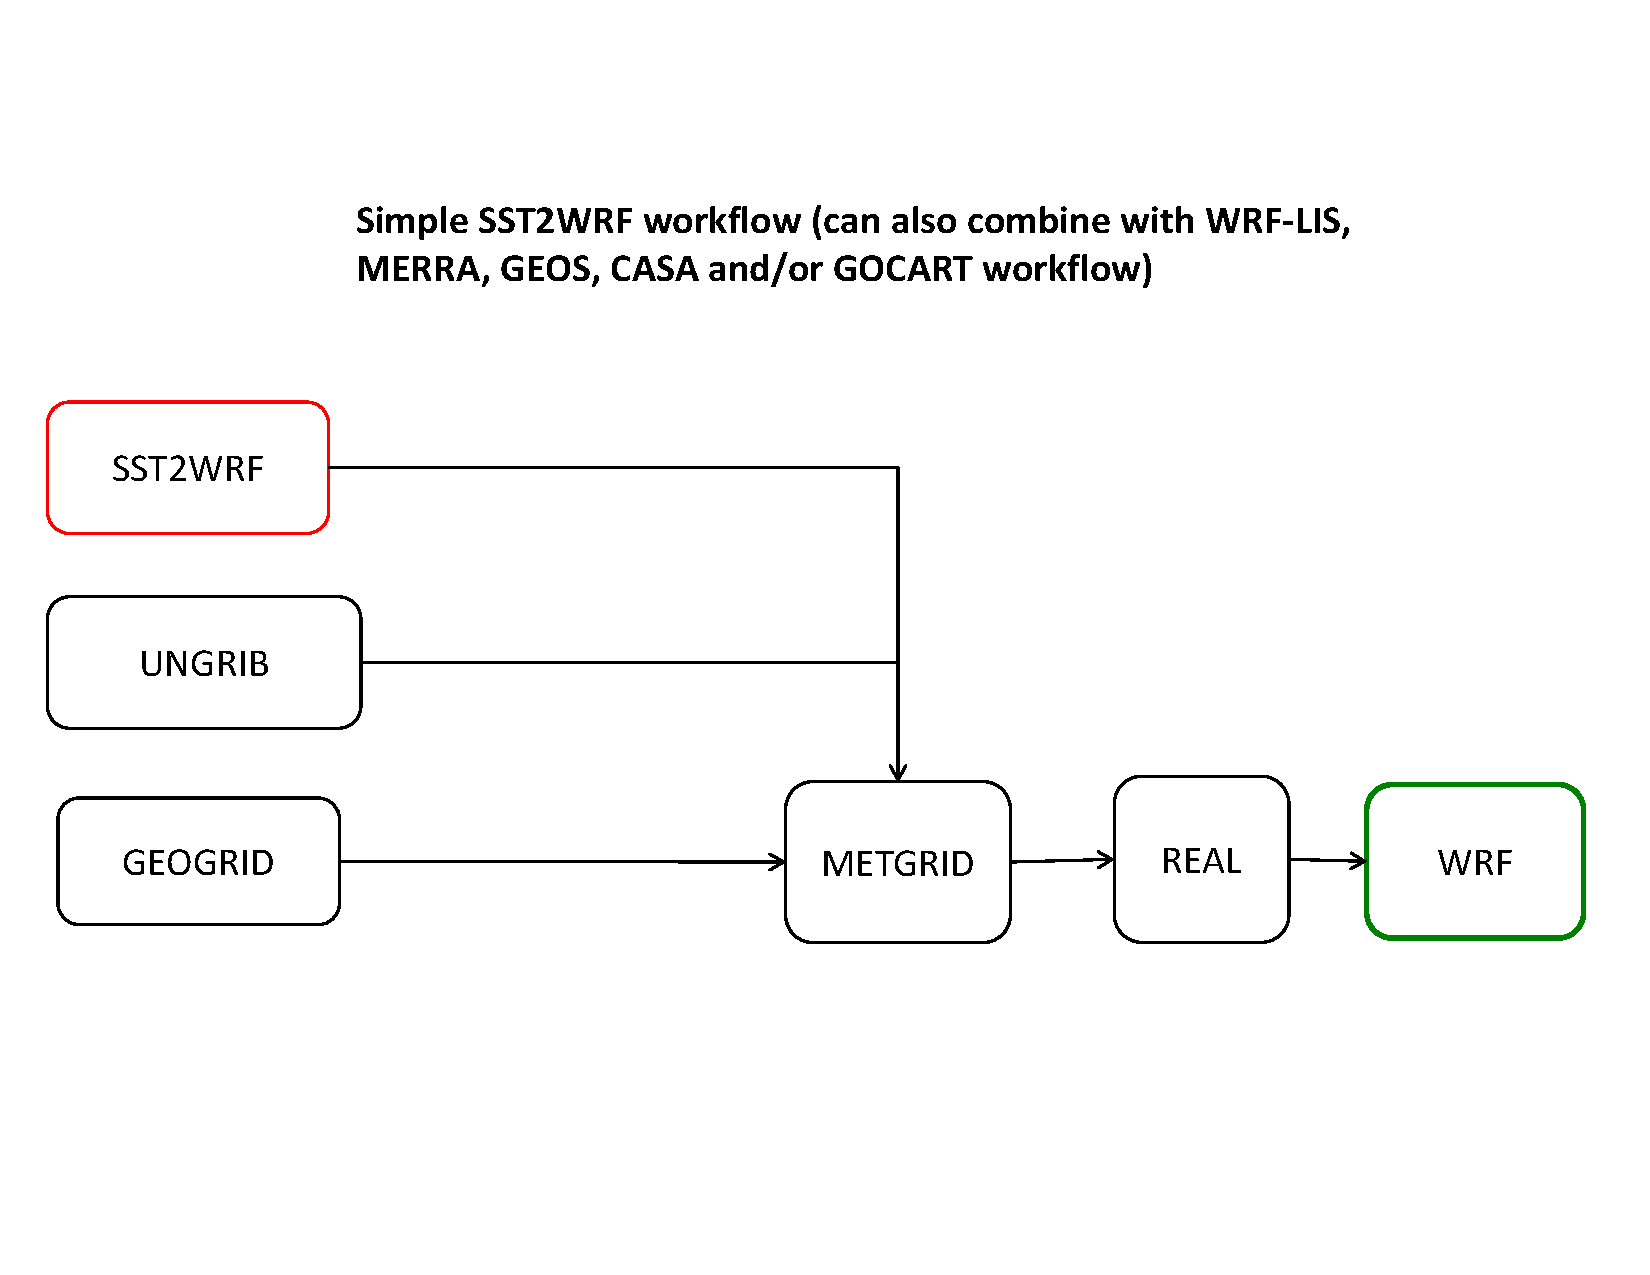
\includegraphics[width=5in]{SST2WRF_workflow}}

\subsection{Initializing Small Inland Lake Temperatures}
\label{subsec:InitLakeTemps}

Proper initialization of lake temperatures can be challenging, as small water
bodies may not be resolved by external datasets (GRIB, MERRA2, RSS SST, etc).
By default, METGRID will extrapolate skin temperature from externally resolved
water points; but this can lead to anomalously warm or cold lake temperatures,
particularly far inland from large water bodies.  To avoid this problem, WPS
provides another approach [from the ``Alternative Initialization of Lake SSTs''
subsection in Chapter 3 of \cite{ref:ArwUserGuide}]:

\begin{itemize}

\item Special landuse datasets (usgs\_lakes and modis\_lakes) that 
discriminate between lakes and oceans.  We recommend using the ``modis\_lakes''
dataset when running GEOGRID.

\item A special preprocessor called AVG\_TSFC, which reads multiple WPS 
intermediate files (from UNGRIB, MERRA2WRF, etc) and calculates daily-average
air temperature (TAVGSFC).  TAVGSFC can then be passed with other data to 
METGRID for horizontal interpolation.  REAL can then use TAVGSFC for the 
surface temperatures over lakes.  While there is room for experimentation, 
feeding data from the previous 4 weeks to AVG\_TSFC should provide reasonable 
estimates for lake temperatures.

\end{itemize}

The attached figure illustrates use of AVG\_TSFC within a simple WRF workflow.
This can be combined with other workflows, including use of SST2WRF; in this 
latter case, the SST field will be used for oceans and large lakes (e.g., the 
Great Lakes), while the TAVGSFC data will be used for small lake temperatures.

\centerline{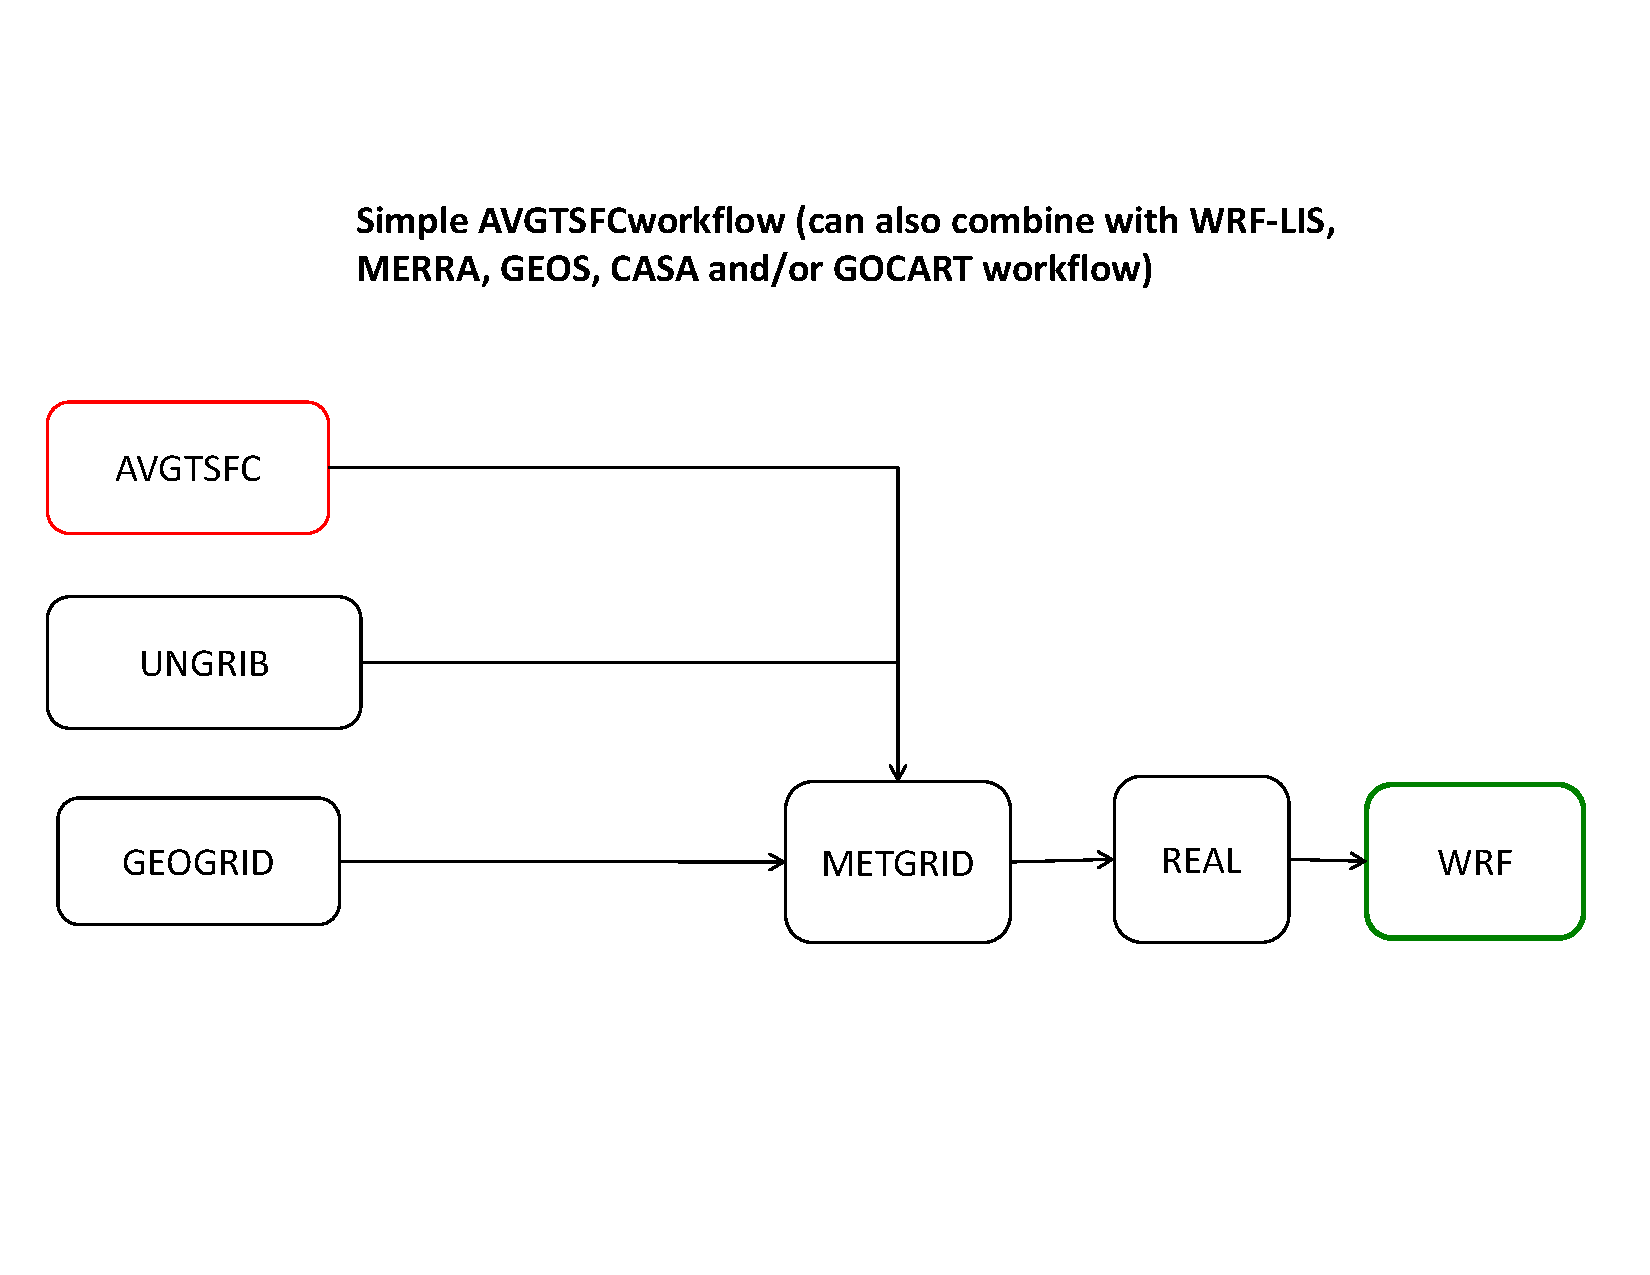
\includegraphics[width=5in]{AVG_TSFC_workflow}}


